% Options for packages loaded elsewhere
\PassOptionsToPackage{unicode}{hyperref}
\PassOptionsToPackage{hyphens}{url}
%
\documentclass[
]{article}
\usepackage{amsmath,amssymb}
\usepackage{lmodern}
\usepackage{ifxetex,ifluatex}
\ifnum 0\ifxetex 1\fi\ifluatex 1\fi=0 % if pdftex
  \usepackage[T1]{fontenc}
  \usepackage[utf8]{inputenc}
  \usepackage{textcomp} % provide euro and other symbols
\else % if luatex or xetex
  \usepackage{unicode-math}
  \defaultfontfeatures{Scale=MatchLowercase}
  \defaultfontfeatures[\rmfamily]{Ligatures=TeX,Scale=1}
\fi
% Use upquote if available, for straight quotes in verbatim environments
\IfFileExists{upquote.sty}{\usepackage{upquote}}{}
\IfFileExists{microtype.sty}{% use microtype if available
  \usepackage[]{microtype}
  \UseMicrotypeSet[protrusion]{basicmath} % disable protrusion for tt fonts
}{}
\makeatletter
\@ifundefined{KOMAClassName}{% if non-KOMA class
  \IfFileExists{parskip.sty}{%
    \usepackage{parskip}
  }{% else
    \setlength{\parindent}{0pt}
    \setlength{\parskip}{6pt plus 2pt minus 1pt}}
}{% if KOMA class
  \KOMAoptions{parskip=half}}
\makeatother
\usepackage{xcolor}
\IfFileExists{xurl.sty}{\usepackage{xurl}}{} % add URL line breaks if available
\IfFileExists{bookmark.sty}{\usepackage{bookmark}}{\usepackage{hyperref}}
\hypersetup{
  pdftitle={Albacore Diet Synthesis B},
  pdfauthor={Natasha Hardy},
  hidelinks,
  pdfcreator={LaTeX via pandoc}}
\urlstyle{same} % disable monospaced font for URLs
\usepackage[margin=1in]{geometry}
\usepackage{color}
\usepackage{fancyvrb}
\newcommand{\VerbBar}{|}
\newcommand{\VERB}{\Verb[commandchars=\\\{\}]}
\DefineVerbatimEnvironment{Highlighting}{Verbatim}{commandchars=\\\{\}}
% Add ',fontsize=\small' for more characters per line
\usepackage{framed}
\definecolor{shadecolor}{RGB}{248,248,248}
\newenvironment{Shaded}{\begin{snugshade}}{\end{snugshade}}
\newcommand{\AlertTok}[1]{\textcolor[rgb]{0.94,0.16,0.16}{#1}}
\newcommand{\AnnotationTok}[1]{\textcolor[rgb]{0.56,0.35,0.01}{\textbf{\textit{#1}}}}
\newcommand{\AttributeTok}[1]{\textcolor[rgb]{0.77,0.63,0.00}{#1}}
\newcommand{\BaseNTok}[1]{\textcolor[rgb]{0.00,0.00,0.81}{#1}}
\newcommand{\BuiltInTok}[1]{#1}
\newcommand{\CharTok}[1]{\textcolor[rgb]{0.31,0.60,0.02}{#1}}
\newcommand{\CommentTok}[1]{\textcolor[rgb]{0.56,0.35,0.01}{\textit{#1}}}
\newcommand{\CommentVarTok}[1]{\textcolor[rgb]{0.56,0.35,0.01}{\textbf{\textit{#1}}}}
\newcommand{\ConstantTok}[1]{\textcolor[rgb]{0.00,0.00,0.00}{#1}}
\newcommand{\ControlFlowTok}[1]{\textcolor[rgb]{0.13,0.29,0.53}{\textbf{#1}}}
\newcommand{\DataTypeTok}[1]{\textcolor[rgb]{0.13,0.29,0.53}{#1}}
\newcommand{\DecValTok}[1]{\textcolor[rgb]{0.00,0.00,0.81}{#1}}
\newcommand{\DocumentationTok}[1]{\textcolor[rgb]{0.56,0.35,0.01}{\textbf{\textit{#1}}}}
\newcommand{\ErrorTok}[1]{\textcolor[rgb]{0.64,0.00,0.00}{\textbf{#1}}}
\newcommand{\ExtensionTok}[1]{#1}
\newcommand{\FloatTok}[1]{\textcolor[rgb]{0.00,0.00,0.81}{#1}}
\newcommand{\FunctionTok}[1]{\textcolor[rgb]{0.00,0.00,0.00}{#1}}
\newcommand{\ImportTok}[1]{#1}
\newcommand{\InformationTok}[1]{\textcolor[rgb]{0.56,0.35,0.01}{\textbf{\textit{#1}}}}
\newcommand{\KeywordTok}[1]{\textcolor[rgb]{0.13,0.29,0.53}{\textbf{#1}}}
\newcommand{\NormalTok}[1]{#1}
\newcommand{\OperatorTok}[1]{\textcolor[rgb]{0.81,0.36,0.00}{\textbf{#1}}}
\newcommand{\OtherTok}[1]{\textcolor[rgb]{0.56,0.35,0.01}{#1}}
\newcommand{\PreprocessorTok}[1]{\textcolor[rgb]{0.56,0.35,0.01}{\textit{#1}}}
\newcommand{\RegionMarkerTok}[1]{#1}
\newcommand{\SpecialCharTok}[1]{\textcolor[rgb]{0.00,0.00,0.00}{#1}}
\newcommand{\SpecialStringTok}[1]{\textcolor[rgb]{0.31,0.60,0.02}{#1}}
\newcommand{\StringTok}[1]{\textcolor[rgb]{0.31,0.60,0.02}{#1}}
\newcommand{\VariableTok}[1]{\textcolor[rgb]{0.00,0.00,0.00}{#1}}
\newcommand{\VerbatimStringTok}[1]{\textcolor[rgb]{0.31,0.60,0.02}{#1}}
\newcommand{\WarningTok}[1]{\textcolor[rgb]{0.56,0.35,0.01}{\textbf{\textit{#1}}}}
\usepackage{graphicx}
\makeatletter
\def\maxwidth{\ifdim\Gin@nat@width>\linewidth\linewidth\else\Gin@nat@width\fi}
\def\maxheight{\ifdim\Gin@nat@height>\textheight\textheight\else\Gin@nat@height\fi}
\makeatother
% Scale images if necessary, so that they will not overflow the page
% margins by default, and it is still possible to overwrite the defaults
% using explicit options in \includegraphics[width, height, ...]{}
\setkeys{Gin}{width=\maxwidth,height=\maxheight,keepaspectratio}
% Set default figure placement to htbp
\makeatletter
\def\fps@figure{htbp}
\makeatother
\setlength{\emergencystretch}{3em} % prevent overfull lines
\providecommand{\tightlist}{%
  \setlength{\itemsep}{0pt}\setlength{\parskip}{0pt}}
\setcounter{secnumdepth}{-\maxdimen} % remove section numbering
\ifluatex
  \usepackage{selnolig}  % disable illegal ligatures
\fi

\title{Albacore Diet Synthesis B}
\author{Natasha Hardy}
\date{15/04/2021}

\begin{document}
\maketitle

\hypertarget{prey-typologies-identified-in-the-diets-of-albacore-tuna}{%
\section{Prey typologies identified in the diets of albacore
tuna}\label{prey-typologies-identified-in-the-diets-of-albacore-tuna}}

\hypertarget{workspace}{%
\subsection{Workspace}\label{workspace}}

\begin{Shaded}
\begin{Highlighting}[]
\CommentTok{\#Need packages}
\FunctionTok{library}\NormalTok{(plyr)}
\FunctionTok{library}\NormalTok{(dplyr)}
\FunctionTok{library}\NormalTok{(tidyverse)}
\FunctionTok{library}\NormalTok{(reshape2)}
\FunctionTok{library}\NormalTok{(factoextra)}
\FunctionTok{library}\NormalTok{(here)}
\StringTok{"\%notin\%"} \OtherTok{=} \FunctionTok{Negate}\NormalTok{(}\StringTok{\textquotesingle{}\%in\%\textquotesingle{}}\NormalTok{)}
\NormalTok{here}\SpecialCharTok{::}\FunctionTok{here}\NormalTok{()}
\end{Highlighting}
\end{Shaded}

\begin{verbatim}
## [1] "/Users/tashhardy/Documents/GitHub/albacore-diet-global"
\end{verbatim}

\begin{Shaded}
\begin{Highlighting}[]
\CommentTok{\#Markdown}
\FunctionTok{library}\NormalTok{(formatR)}

\CommentTok{\# Graphics}
\FunctionTok{library}\NormalTok{(ggplot2)}
\FunctionTok{library}\NormalTok{(}\StringTok{"PNWColors"}\NormalTok{)}
\FunctionTok{library}\NormalTok{(viridis)}

\CommentTok{\#Multivariate work}
\FunctionTok{library}\NormalTok{(vegan)}
\FunctionTok{library}\NormalTok{(cluster)}
\FunctionTok{library}\NormalTok{(}\StringTok{"dendextend"}\NormalTok{)}
\FunctionTok{library}\NormalTok{(NbClust)}
\end{Highlighting}
\end{Shaded}

\hypertarget{probable-prey-traits-load-cluster-algorithms}{%
\subsection{PROBABLE prey traits load \& cluster
algorithms}\label{probable-prey-traits-load-cluster-algorithms}}

\hypertarget{prey-traits-for-cluster--}{%
\subsubsection{Prey \& traits for cluster
----}\label{prey-traits-for-cluster--}}

\begin{Shaded}
\begin{Highlighting}[]
\NormalTok{prey\_probable\_load }\OtherTok{=} \FunctionTok{read.csv}\NormalTok{(}\FunctionTok{here}\NormalTok{(}\StringTok{"data/output\_data/prey\_probable\_traits.csv"}\NormalTok{),}
    \AttributeTok{header =} \ConstantTok{TRUE}\NormalTok{) }\SpecialCharTok{\%\textgreater{}\%}
\NormalTok{    dplyr}\SpecialCharTok{::}\FunctionTok{select}\NormalTok{(}\SpecialCharTok{{-}}\FunctionTok{c}\NormalTok{(X, diel\_migrant, refuge, season\_migrant, l\_max, trophic\_level}\SpecialCharTok{:}\NormalTok{standard\_total,}
\NormalTok{        energy\_density}\SpecialCharTok{:}\NormalTok{percent\_lipid)) }\SpecialCharTok{\%\textgreater{}\%}
\NormalTok{    dplyr}\SpecialCharTok{::}\FunctionTok{rename}\NormalTok{(}\AttributeTok{gregarious =}\NormalTok{ gregarious\_primary) }\SpecialCharTok{\%\textgreater{}\%}
    \FunctionTok{mutate}\NormalTok{(}\AttributeTok{diel\_migrant\_cat =} \FunctionTok{case\_when}\NormalTok{(diel\_migrant\_cat }\SpecialCharTok{==} \StringTok{"diel\_no"} \SpecialCharTok{\textasciitilde{}} \StringTok{"diel (no)"}\NormalTok{,}
\NormalTok{        diel\_migrant\_cat }\SpecialCharTok{==} \StringTok{"diel\_UN"} \SpecialCharTok{\textasciitilde{}} \StringTok{"diel (unknown)"}\NormalTok{, diel\_migrant\_cat }\SpecialCharTok{==} \StringTok{"diel\_yes"} \SpecialCharTok{\textasciitilde{}}
            \StringTok{"diel (yes)"}\NormalTok{), }\AttributeTok{refuge\_cat =} \FunctionTok{case\_when}\NormalTok{(refuge\_cat }\SpecialCharTok{==} \StringTok{"refuge\_no"} \SpecialCharTok{\textasciitilde{}} \StringTok{"refuge (no)"}\NormalTok{,}
\NormalTok{        refuge\_cat }\SpecialCharTok{==} \StringTok{"refuge\_NA"} \SpecialCharTok{\textasciitilde{}} \StringTok{"refuge (unknown)"}\NormalTok{, refuge\_cat }\SpecialCharTok{==} \StringTok{"refuge\_yes"} \SpecialCharTok{\textasciitilde{}}
            \StringTok{"refuge (yes)"}\NormalTok{), }\AttributeTok{gregarious =} \FunctionTok{case\_when}\NormalTok{(gregarious }\SpecialCharTok{==} \StringTok{"solitary"} \SpecialCharTok{\textasciitilde{}} \StringTok{"solitary"}\NormalTok{,}
\NormalTok{        gregarious }\SpecialCharTok{==} \StringTok{"pairing"} \SpecialCharTok{\textasciitilde{}} \StringTok{"solitary"}\NormalTok{, gregarious }\SpecialCharTok{==} \StringTok{"shoaling"} \SpecialCharTok{\textasciitilde{}} \StringTok{"schooling"}\NormalTok{,}
\NormalTok{        gregarious }\SpecialCharTok{==} \StringTok{"schooling"} \SpecialCharTok{\textasciitilde{}} \StringTok{"schooling"}\NormalTok{), }\AttributeTok{season\_cat =} \FunctionTok{case\_when}\NormalTok{(season\_cat }\SpecialCharTok{==}
        \StringTok{"season\_no"} \SpecialCharTok{\textasciitilde{}} \StringTok{"season (no)"}\NormalTok{, season\_cat }\SpecialCharTok{==} \StringTok{"season\_NA"} \SpecialCharTok{\textasciitilde{}} \StringTok{"season (unknown)"}\NormalTok{,}
\NormalTok{        season\_cat }\SpecialCharTok{==} \StringTok{"season\_yes"} \SpecialCharTok{\textasciitilde{}} \StringTok{"season (yes)"}\NormalTok{))}

\NormalTok{prey\_probable }\OtherTok{=}\NormalTok{ prey\_probable\_load }\SpecialCharTok{\%\textgreater{}\%}
    \FunctionTok{filter}\NormalTok{(diel\_migrant\_cat }\SpecialCharTok{!=} \StringTok{"diel (unknown)"}\NormalTok{, refuge\_cat }\SpecialCharTok{!=} \StringTok{"refuge (unknown)"}\NormalTok{,}
\NormalTok{        season\_cat }\SpecialCharTok{!=} \StringTok{"season (unknown)"}\NormalTok{) }\SpecialCharTok{\%\textgreater{}\%}
    \FunctionTok{drop\_na}\NormalTok{()}
\CommentTok{\# reduced from \textasciitilde{}298 taxa to \textasciitilde{}156 levels(as.factor(prey\_probable$gregarious))}

\FunctionTok{summary}\NormalTok{(prey\_probable)}
\end{Highlighting}
\end{Shaded}

\begin{verbatim}
##   prey_class         prey_order        prey_family          prey_sp         
##  Length:156         Length:156         Length:156         Length:156        
##  Class :character   Class :character   Class :character   Class :character  
##  Mode  :character   Mode  :character   Mode  :character   Mode  :character  
##                                                                             
##                                                                             
##                                                                             
##   life_stage        vert_habitat       horz_habitat       diel_migrant_cat  
##  Length:156         Length:156         Length:156         Length:156        
##  Class :character   Class :character   Class :character   Class :character  
##  Mode  :character   Mode  :character   Mode  :character   Mode  :character  
##                                                                             
##                                                                             
##                                                                             
##   refuge_cat         season_cat         body_shape         phys_defense   
##  Length:156         Length:156         Length:156         Min.   :0.0000  
##  Class :character   Class :character   Class :character   1st Qu.:0.0000  
##  Mode  :character   Mode  :character   Mode  :character   Median :0.0000  
##                                                           Mean   :0.4295  
##                                                           3rd Qu.:1.0000  
##                                                           Max.   :1.0000  
##   transparent     col_disrupt         silver        countershade   
##  Min.   :0.000   Min.   :0.0000   Min.   :0.0000   Min.   :0.0000  
##  1st Qu.:0.000   1st Qu.:0.0000   1st Qu.:0.0000   1st Qu.:0.0000  
##  Median :0.000   Median :0.0000   Median :0.0000   Median :0.0000  
##  Mean   :0.109   Mean   :0.4551   Mean   :0.4231   Mean   :0.3205  
##  3rd Qu.:0.000   3rd Qu.:1.0000   3rd Qu.:1.0000   3rd Qu.:1.0000  
##  Max.   :1.000   Max.   :1.0000   Max.   :1.0000   Max.   :1.0000  
##   gregarious            maxFO              maxN             maxM       
##  Length:156         Min.   :  0.000   Min.   : 0.000   Min.   : 0.000  
##  Class :character   1st Qu.:  1.500   1st Qu.: 0.000   1st Qu.: 0.000  
##  Mode  :character   Median :  5.578   Median : 0.100   Median : 0.000  
##                     Mean   : 17.620   Mean   : 4.505   Mean   : 5.054  
##                     3rd Qu.: 28.200   3rd Qu.: 1.613   3rd Qu.: 2.250  
##                     Max.   :100.000   Max.   :78.500   Max.   :95.200
\end{verbatim}

\begin{Shaded}
\begin{Highlighting}[]
\DocumentationTok{\#\# Row name as column datasets For probable prey traits}
\NormalTok{prey\_probable\_row }\OtherTok{\textless{}{-}}\NormalTok{ prey\_probable}
\NormalTok{dendlabs }\OtherTok{\textless{}{-}} \FunctionTok{rownames}\NormalTok{(prey\_probable\_row)}
\NormalTok{prey\_probable }\OtherTok{\textless{}{-}} \FunctionTok{cbind}\NormalTok{(dendlabs, prey\_probable\_row)}

\CommentTok{\# Probable trait df subsets}
\NormalTok{probable\_species }\OtherTok{=}\NormalTok{ prey\_probable}\SpecialCharTok{$}\NormalTok{prey\_sp}
\NormalTok{prey\_probable[, }\DecValTok{6}\SpecialCharTok{:}\DecValTok{17}\NormalTok{] }\OtherTok{=} \FunctionTok{lapply}\NormalTok{(prey\_probable[, }\DecValTok{6}\SpecialCharTok{:}\DecValTok{17}\NormalTok{], as.factor)}
\NormalTok{probable\_traits }\OtherTok{=} \FunctionTok{as.data.frame}\NormalTok{(prey\_probable[, }\FunctionTok{c}\NormalTok{(}\DecValTok{6}\SpecialCharTok{:}\DecValTok{10}\NormalTok{, }\DecValTok{11}\NormalTok{)])  }\CommentTok{\#12}

\NormalTok{probable\_traits }\OtherTok{=}\NormalTok{ prey\_probable }\SpecialCharTok{\%\textgreater{}\%}
\NormalTok{    dplyr}\SpecialCharTok{::}\FunctionTok{select}\NormalTok{(life\_stage, vert\_habitat, horz\_habitat, diel\_migrant\_cat, season\_cat)}

\FunctionTok{str}\NormalTok{(probable\_traits)}
\end{Highlighting}
\end{Shaded}

\begin{verbatim}
## 'data.frame':    156 obs. of  5 variables:
##  $ life_stage      : Factor w/ 3 levels "adult","juvenile",..: 1 1 1 2 2 1 1 1 1 1 ...
##  $ vert_habitat    : Factor w/ 5 levels "bathypelagic",..: 5 2 4 3 4 5 4 4 5 2 ...
##  $ horz_habitat    : Factor w/ 5 levels "coastal","continental shelf",..: 4 1 2 2 2 4 4 4 4 2 ...
##  $ diel_migrant_cat: Factor w/ 2 levels "diel (no)","diel (yes)": 2 2 2 2 1 2 1 1 2 2 ...
##  $ season_cat      : Factor w/ 2 levels "season (no)",..: 2 1 2 2 2 2 2 2 1 2 ...
\end{verbatim}

\hypertarget{cluster-techniques--}{%
\subsubsection{Cluster techniques ----}\label{cluster-techniques--}}

\begin{Shaded}
\begin{Highlighting}[]
\DocumentationTok{\#\#\#\# Distance measure {-}{-}{-}{-}}
\CommentTok{\#select just the traits you want to contribute to ordination}
\NormalTok{prob.gower.dist }\OtherTok{\textless{}{-}} \FunctionTok{daisy}\NormalTok{(probable\_traits, }\AttributeTok{metric =} \FunctionTok{c}\NormalTok{(}\StringTok{"gower"}\NormalTok{))}

\DocumentationTok{\#\#\#\# Divisive cluster {-}{-}{-}{-}}
\NormalTok{prob.divisive.clust }\OtherTok{\textless{}{-}} \FunctionTok{diana}\NormalTok{(}\FunctionTok{as.matrix}\NormalTok{(prob.gower.dist), }
                              \AttributeTok{diss =} \ConstantTok{TRUE}\NormalTok{, }\AttributeTok{keep.diss =} \ConstantTok{TRUE}\NormalTok{)}
\FunctionTok{plot}\NormalTok{(prob.divisive.clust, }\AttributeTok{main =} \StringTok{"Divisive"}\NormalTok{)}
\end{Highlighting}
\end{Shaded}

\includegraphics{Albacore_synthesis_b_files/figure-latex/Cluster \& Dissimilarity Matrix-1.pdf}
\includegraphics{Albacore_synthesis_b_files/figure-latex/Cluster \& Dissimilarity Matrix-2.pdf}

\begin{Shaded}
\begin{Highlighting}[]
\DocumentationTok{\#\#\#\# Agglomerative cluster {-}{-}{-}{-}}
\CommentTok{\#Use "average" or "complete" linkage}
\CommentTok{\#ADD }\AlertTok{NOTE}\CommentTok{ ON AVE VS. COMPLETE LINKAGE}
\NormalTok{prob.aggl.clustc }\OtherTok{\textless{}{-}} \FunctionTok{hclust}\NormalTok{(prob.gower.dist, }\AttributeTok{method =} \StringTok{"complete"}\NormalTok{)}
\FunctionTok{plot}\NormalTok{(prob.aggl.clustc, }\AttributeTok{main =} \StringTok{"Agglomerative, complete linkages"}\NormalTok{)}
\end{Highlighting}
\end{Shaded}

\includegraphics{Albacore_synthesis_b_files/figure-latex/Cluster \& Dissimilarity Matrix-3.pdf}

\begin{Shaded}
\begin{Highlighting}[]
\DocumentationTok{\#\#\#\# nMDS for dissimilarity {-} checking the dissimilarity matrix}
\CommentTok{\#trait\_NMDS\_prob \textless{}{-} metaMDS(prob.gower.dist, trymax = 100)}
\CommentTok{\#trait\_NMDS\_prob[["stress"]] \#stress = 0.1177472}

\CommentTok{\#Plot {-}{-}\textgreater{} }
\CommentTok{\#plot(trait\_NMDS\_prob) \#plots species as black dots, traits as red crosses }
\DocumentationTok{\#\#\#Why are species scores not available?}

\CommentTok{\#Note that the ordination looks good!}
\CommentTok{\#Need to revisit this and plot in relation to clusters!}
\end{Highlighting}
\end{Shaded}

\hypertarget{cluster-assessment-output}{%
\subsubsection{Cluster Assessment
Output}\label{cluster-assessment-output}}

\textbf{Notes} 20-24/07/2020 Ultimately we are aiming for distinct
clusters of species, such that the difference within clusters is minimal
and between clusters is maximised. Assessing cluster statistical tables,
we are consistently observing lower average.within cluster differences
using agglomerative clustering compared to divisive algorithms.
Additionally, cluster sizes and balance are consistently more even using
agglomerative vs.~divisive.

Using habitat use + gregarious (binary) traits, selecting: (i) Divisive
DONT USE (ii) Agglomerative (complete) \#8 clusters (based on balanced
clusters +optimal avg.silwidth value)

Using all traits (habitat use, gregarious, body shape and physical
defenses) (i) Divisive - DO NOT USE (ii) Agglomerative - 10-11 clusters
(based on balanced clusters + optimal avg.silwidth value)

\begin{Shaded}
\begin{Highlighting}[]
\CommentTok{\# Cluster stats comes out as list while it is more convenient to look at it as a table}
\CommentTok{\# This code below will produce a dataframe with observations in columns and variables in row}
\CommentTok{\# Not quite tidy data, which will require a tweak for plotting, but I prefer this view as an output here as I find it more comprehensive }
\FunctionTok{library}\NormalTok{(fpc)}
\NormalTok{cstats.table }\OtherTok{\textless{}{-}} \ControlFlowTok{function}\NormalTok{(dist, tree, k) \{}
\NormalTok{  clust.assess }\OtherTok{\textless{}{-}} \FunctionTok{c}\NormalTok{(}\StringTok{"cluster.number"}\NormalTok{,}\StringTok{"n"}\NormalTok{,}\StringTok{"within.cluster.ss"}\NormalTok{,}\StringTok{"average.within"}\NormalTok{,}\StringTok{"average.between"}\NormalTok{,}
                    \StringTok{"wb.ratio"}\NormalTok{,}\StringTok{"dunn2"}\NormalTok{,}\StringTok{"avg.silwidth"}\NormalTok{)}
\NormalTok{  clust.size }\OtherTok{\textless{}{-}} \FunctionTok{c}\NormalTok{(}\StringTok{"cluster.size"}\NormalTok{)}
\NormalTok{  stats.names }\OtherTok{\textless{}{-}} \FunctionTok{c}\NormalTok{()}
\NormalTok{  row.clust }\OtherTok{\textless{}{-}} \FunctionTok{c}\NormalTok{()}
\NormalTok{  output.stats }\OtherTok{\textless{}{-}} \FunctionTok{matrix}\NormalTok{(}\AttributeTok{ncol =}\NormalTok{ k, }\AttributeTok{nrow =} \FunctionTok{length}\NormalTok{(clust.assess))}
\NormalTok{  cluster.sizes }\OtherTok{\textless{}{-}} \FunctionTok{matrix}\NormalTok{(}\AttributeTok{ncol =}\NormalTok{ k, }\AttributeTok{nrow =}\NormalTok{ k)}
  \ControlFlowTok{for}\NormalTok{(i }\ControlFlowTok{in} \FunctionTok{c}\NormalTok{(}\DecValTok{1}\SpecialCharTok{:}\NormalTok{k))\{}
\NormalTok{    row.clust[i] }\OtherTok{\textless{}{-}} \FunctionTok{paste}\NormalTok{(}\StringTok{"Cluster{-}"}\NormalTok{, i, }\StringTok{" size"}\NormalTok{)}
\NormalTok{  \}}
  \ControlFlowTok{for}\NormalTok{(i }\ControlFlowTok{in} \FunctionTok{c}\NormalTok{(}\DecValTok{2}\SpecialCharTok{:}\NormalTok{k))\{}
\NormalTok{    stats.names[i] }\OtherTok{\textless{}{-}} \FunctionTok{paste}\NormalTok{(}\StringTok{"Test"}\NormalTok{, i}\DecValTok{{-}1}\NormalTok{)}
    
    \ControlFlowTok{for}\NormalTok{(j }\ControlFlowTok{in} \FunctionTok{seq\_along}\NormalTok{(clust.assess))\{}
\NormalTok{      output.stats[j, i] }\OtherTok{\textless{}{-}} \FunctionTok{unlist}\NormalTok{(}\FunctionTok{cluster.stats}\NormalTok{(}\AttributeTok{d =}\NormalTok{ dist, }\AttributeTok{clustering =} \FunctionTok{cutree}\NormalTok{(tree, }\AttributeTok{k =}\NormalTok{ i))[clust.assess])[j]}
      
\NormalTok{    \}}
    
    \ControlFlowTok{for}\NormalTok{(d }\ControlFlowTok{in} \DecValTok{1}\SpecialCharTok{:}\NormalTok{k) \{}
\NormalTok{      cluster.sizes[d, i] }\OtherTok{\textless{}{-}} \FunctionTok{unlist}\NormalTok{(}\FunctionTok{cluster.stats}\NormalTok{(}\AttributeTok{d =}\NormalTok{ dist, }\AttributeTok{clustering =} \FunctionTok{cutree}\NormalTok{(tree, }\AttributeTok{k =}\NormalTok{ i))[clust.size])[d]}
      \FunctionTok{dim}\NormalTok{(cluster.sizes[d, i]) }\OtherTok{\textless{}{-}} \FunctionTok{c}\NormalTok{(}\FunctionTok{length}\NormalTok{(cluster.sizes[i]), }\DecValTok{1}\NormalTok{)}
\NormalTok{      cluster.sizes[d, i]}
      
\NormalTok{    \}}
\NormalTok{  \}}
\NormalTok{  output.stats.df }\OtherTok{\textless{}{-}} \FunctionTok{data.frame}\NormalTok{(output.stats)}
\NormalTok{  cluster.sizes }\OtherTok{\textless{}{-}} \FunctionTok{data.frame}\NormalTok{(cluster.sizes)}
\NormalTok{  cluster.sizes[}\FunctionTok{is.na}\NormalTok{(cluster.sizes)] }\OtherTok{\textless{}{-}} \DecValTok{0}
\NormalTok{  rows.all }\OtherTok{\textless{}{-}} \FunctionTok{c}\NormalTok{(clust.assess, row.clust)}
  \CommentTok{\# rownames(output.stats.df) \textless{}{-} clust.assess}
\NormalTok{  output }\OtherTok{\textless{}{-}} \FunctionTok{rbind}\NormalTok{(output.stats.df, cluster.sizes)[ ,}\SpecialCharTok{{-}}\DecValTok{1}\NormalTok{]}
  \FunctionTok{colnames}\NormalTok{(output) }\OtherTok{\textless{}{-}}\NormalTok{ stats.names[}\DecValTok{2}\SpecialCharTok{:}\NormalTok{k]}
  \FunctionTok{rownames}\NormalTok{(output) }\OtherTok{\textless{}{-}}\NormalTok{ rows.all}
\NormalTok{  is.num }\OtherTok{\textless{}{-}} \FunctionTok{sapply}\NormalTok{(output, is.numeric)}
\NormalTok{  output[is.num] }\OtherTok{\textless{}{-}} \FunctionTok{lapply}\NormalTok{(output[is.num], round, }\DecValTok{2}\NormalTok{)}
\NormalTok{  output}
\NormalTok{\}}
\end{Highlighting}
\end{Shaded}

\begin{Shaded}
\begin{Highlighting}[]
\CommentTok{\#Stats table for divisive method}
\NormalTok{prob.stats.df.divisive }\OtherTok{\textless{}{-}} \FunctionTok{cstats.table}\NormalTok{(prob.gower.dist, prob.divisive.clust, }\DecValTok{15}\NormalTok{)}
\NormalTok{prob.stats.df.divisive}
\end{Highlighting}
\end{Shaded}

\begin{verbatim}
##                   Test 1 Test 2 Test 3 Test 4 Test 5 Test 6 Test 7 Test 8
## cluster.number      2.00   3.00   4.00   5.00   6.00   7.00   8.00   9.00
## n                 156.00 156.00 156.00 156.00 156.00 156.00 156.00 156.00
## within.cluster.ss  18.54  14.87  12.66  10.30   9.45   7.73   7.46   6.93
## average.within      0.44   0.39   0.37   0.31   0.29   0.26   0.25   0.24
## average.between     0.65   0.63   0.63   0.59   0.59   0.58   0.58   0.58
## wb.ratio            0.68   0.62   0.58   0.53   0.50   0.44   0.43   0.42
## dunn2               1.40   1.27   1.35   1.06   0.77   0.77   0.77   0.77
## avg.silwidth        0.32   0.30   0.32   0.30   0.24   0.30   0.28   0.29
## Cluster- 1  size  107.00  86.00  86.00  31.00  31.00  31.00  31.00  31.00
## Cluster- 2  size   49.00  49.00  36.00  36.00  36.00  36.00  36.00  36.00
## Cluster- 3  size    0.00  21.00  21.00  55.00  47.00  26.00  22.00  22.00
## Cluster- 4  size    0.00   0.00  13.00  21.00  21.00  21.00  21.00  11.00
## Cluster- 5  size    0.00   0.00   0.00  13.00   8.00   8.00   4.00   4.00
## Cluster- 6  size    0.00   0.00   0.00   0.00  13.00  21.00   8.00   8.00
## Cluster- 7  size    0.00   0.00   0.00   0.00   0.00  13.00  21.00  21.00
## Cluster- 8  size    0.00   0.00   0.00   0.00   0.00   0.00  13.00  13.00
## Cluster- 9  size    0.00   0.00   0.00   0.00   0.00   0.00   0.00  10.00
## Cluster- 10  size   0.00   0.00   0.00   0.00   0.00   0.00   0.00   0.00
## Cluster- 11  size   0.00   0.00   0.00   0.00   0.00   0.00   0.00   0.00
## Cluster- 12  size   0.00   0.00   0.00   0.00   0.00   0.00   0.00   0.00
## Cluster- 13  size   0.00   0.00   0.00   0.00   0.00   0.00   0.00   0.00
## Cluster- 14  size   0.00   0.00   0.00   0.00   0.00   0.00   0.00   0.00
## Cluster- 15  size   0.00   0.00   0.00   0.00   0.00   0.00   0.00   0.00
##                   Test 9 Test 10 Test 11 Test 12 Test 13 Test 14
## cluster.number     10.00   11.00   12.00   13.00   14.00   15.00
## n                 156.00  156.00  156.00  156.00  156.00  156.00
## within.cluster.ss   6.68    6.50    5.47    4.80    4.56    3.97
## average.within      0.24    0.23    0.21    0.20    0.19    0.18
## average.between     0.58    0.58    0.57    0.57    0.57    0.57
## wb.ratio            0.41    0.40    0.37    0.35    0.34    0.32
## dunn2               0.77    0.77    0.77    0.77    0.76    1.06
## avg.silwidth        0.28    0.28    0.33    0.37    0.37    0.39
## Cluster- 1  size   31.00   31.00   31.00   31.00   31.00   31.00
## Cluster- 2  size   36.00   36.00   11.00   11.00   11.00   11.00
## Cluster- 3  size   22.00   22.00   22.00   22.00   22.00   22.00
## Cluster- 4  size   11.00   11.00   11.00   11.00   11.00   11.00
## Cluster- 5  size    4.00    4.00   25.00   16.00   16.00   16.00
## Cluster- 6  size    8.00    8.00    4.00    4.00    4.00    4.00
## Cluster- 7  size   21.00   21.00    8.00    8.00    8.00    8.00
## Cluster- 8  size   13.00   13.00   21.00    9.00    9.00    9.00
## Cluster- 9  size    8.00    6.00   13.00   21.00   21.00   21.00
## Cluster- 10  size   2.00    2.00    6.00   13.00    3.00    3.00
## Cluster- 11  size   0.00    2.00    2.00    6.00    6.00    6.00
## Cluster- 12  size   0.00    0.00    2.00    2.00    2.00    2.00
## Cluster- 13  size   0.00    0.00    0.00    2.00   10.00    5.00
## Cluster- 14  size   0.00    0.00    0.00    0.00    2.00    5.00
## Cluster- 15  size   0.00    0.00    0.00    0.00    0.00    2.00
\end{verbatim}

\begin{Shaded}
\begin{Highlighting}[]
\FunctionTok{View}\NormalTok{(prob.stats.df.divisive)}
\FunctionTok{write.csv}\NormalTok{(prob.stats.df.divisive, }\FunctionTok{here}\NormalTok{(}\StringTok{"outputs\_figures/clusters/prob.stats.df.divisive.csv"}\NormalTok{))}

\CommentTok{\#Stats table for agglomerative method}
\NormalTok{prob.stats.df.aggl }\OtherTok{\textless{}{-}} \FunctionTok{cstats.table}\NormalTok{(prob.gower.dist, prob.aggl.clustc, }\DecValTok{15}\NormalTok{) }
\CommentTok{\#complete linkages looks like the most balanced approach}
\NormalTok{prob.stats.df.aggl}
\end{Highlighting}
\end{Shaded}

\begin{verbatim}
##                   Test 1 Test 2 Test 3 Test 4 Test 5 Test 6 Test 7 Test 8
## cluster.number      2.00   3.00   4.00   5.00   6.00   7.00   8.00   9.00
## n                 156.00 156.00 156.00 156.00 156.00 156.00 156.00 156.00
## within.cluster.ss  21.97  17.51  15.73  15.38  14.73  13.46   9.65   9.41
## average.within      0.47   0.42   0.40   0.39   0.38   0.36   0.31   0.30
## average.between     0.58   0.61   0.61   0.61   0.61   0.60   0.59   0.59
## wb.ratio            0.82   0.69   0.65   0.64   0.63   0.60   0.52   0.51
## dunn2               1.12   1.18   1.12   1.02   0.88   0.92   0.92   0.83
## avg.silwidth        0.17   0.21   0.19   0.15   0.14   0.15   0.26   0.23
## Cluster- 1  size  108.00  92.00  92.00  92.00  92.00  83.00  50.00  50.00
## Cluster- 2  size   48.00  16.00  16.00  12.00   8.00   8.00   8.00   8.00
## Cluster- 3  size    0.00  48.00  40.00  40.00  40.00  40.00  33.00  33.00
## Cluster- 4  size    0.00   0.00   8.00   8.00   8.00   9.00  40.00  40.00
## Cluster- 5  size    0.00   0.00   0.00   4.00   4.00   8.00   9.00   9.00
## Cluster- 6  size    0.00   0.00   0.00   0.00   4.00   4.00   8.00   6.00
## Cluster- 7  size    0.00   0.00   0.00   0.00   0.00   4.00   4.00   4.00
## Cluster- 8  size    0.00   0.00   0.00   0.00   0.00   0.00   4.00   2.00
## Cluster- 9  size    0.00   0.00   0.00   0.00   0.00   0.00   0.00   4.00
## Cluster- 10  size   0.00   0.00   0.00   0.00   0.00   0.00   0.00   0.00
## Cluster- 11  size   0.00   0.00   0.00   0.00   0.00   0.00   0.00   0.00
## Cluster- 12  size   0.00   0.00   0.00   0.00   0.00   0.00   0.00   0.00
## Cluster- 13  size   0.00   0.00   0.00   0.00   0.00   0.00   0.00   0.00
## Cluster- 14  size   0.00   0.00   0.00   0.00   0.00   0.00   0.00   0.00
## Cluster- 15  size   0.00   0.00   0.00   0.00   0.00   0.00   0.00   0.00
##                   Test 9 Test 10 Test 11 Test 12 Test 13 Test 14
## cluster.number     10.00   11.00   12.00   13.00   14.00   15.00
## n                 156.00  156.00  156.00  156.00  156.00  156.00
## within.cluster.ss   9.21    8.18    6.47    5.98    5.46    3.88
## average.within      0.30    0.28    0.24    0.23    0.22    0.19
## average.between     0.59    0.59    0.58    0.58    0.58    0.57
## wb.ratio            0.50    0.47    0.41    0.40    0.38    0.32
## dunn2               0.83    0.83    0.82    1.15    1.26    1.30
## avg.silwidth        0.19    0.20    0.28    0.29    0.30    0.41
## Cluster- 1  size   50.00   50.00   50.00   50.00   47.00   30.00
## Cluster- 2  size    8.00    8.00    8.00    4.00    4.00    4.00
## Cluster- 3  size   33.00   33.00   14.00   14.00   14.00   17.00
## Cluster- 4  size   39.00   29.00   29.00   29.00   29.00   14.00
## Cluster- 5  size    9.00   10.00   10.00   10.00   10.00   29.00
## Cluster- 6  size    6.00    9.00    9.00    9.00    9.00   10.00
## Cluster- 7  size    4.00    6.00   19.00   19.00   19.00    9.00
## Cluster- 8  size    2.00    4.00    6.00    4.00    4.00   19.00
## Cluster- 9  size    4.00    2.00    4.00    6.00    6.00    4.00
## Cluster- 10  size   1.00    4.00    2.00    4.00    4.00    6.00
## Cluster- 11  size   0.00    1.00    4.00    2.00    3.00    4.00
## Cluster- 12  size   0.00    0.00    1.00    4.00    2.00    3.00
## Cluster- 13  size   0.00    0.00    0.00    1.00    4.00    2.00
## Cluster- 14  size   0.00    0.00    0.00    0.00    1.00    4.00
## Cluster- 15  size   0.00    0.00    0.00    0.00    0.00    1.00
\end{verbatim}

\begin{Shaded}
\begin{Highlighting}[]
\FunctionTok{View}\NormalTok{(prob.stats.df.aggl)}
\FunctionTok{write.csv}\NormalTok{(prob.stats.df.aggl, }\FunctionTok{here}\NormalTok{(}\StringTok{"outputs\_figures/clusters/prob.stats.df.aggl.csv"}\NormalTok{))}
\CommentTok{\#As per text for adult, average within cluster metric is minimised for \textasciitilde{}7{-}10 clusters, and the average between for about the same. The agglomerative clustering appears more balanced.}
\end{Highlighting}
\end{Shaded}

\textbf{Note} Agglomerative -- for visualising cluster number selection.

Currently not using the agglomerative output based on stats table
output.

\begin{Shaded}
\begin{Highlighting}[]
\DocumentationTok{\#\#\# Using "Elbow" and "Silhouette" methods to identify the best number of clusters}

\CommentTok{\# Elbow method}

\CommentTok{\# Agglomerative clustering,provides a more ambiguous picture}
\FunctionTok{ggplot}\NormalTok{(}\AttributeTok{data =} \FunctionTok{data.frame}\NormalTok{(}\FunctionTok{t}\NormalTok{(}\FunctionTok{cstats.table}\NormalTok{(prob.gower.dist, prob.aggl.clustc, }\DecValTok{20}\NormalTok{))), }
       \FunctionTok{aes}\NormalTok{(}\AttributeTok{x=}\NormalTok{cluster.number, }\AttributeTok{y=}\NormalTok{within.cluster.ss)) }\SpecialCharTok{+} 
  \FunctionTok{geom\_point}\NormalTok{()}\SpecialCharTok{+}
  \FunctionTok{geom\_line}\NormalTok{()}\SpecialCharTok{+}
  \FunctionTok{ggtitle}\NormalTok{(}\StringTok{"Agglomerative clustering"}\NormalTok{) }\SpecialCharTok{+}
  \FunctionTok{labs}\NormalTok{(}\AttributeTok{x =} \StringTok{"Num.of clusters"}\NormalTok{, }\AttributeTok{y =} \StringTok{"Within clusters sum of squares (SS)"}\NormalTok{) }\SpecialCharTok{+}
  \FunctionTok{theme}\NormalTok{(}\AttributeTok{plot.title =} \FunctionTok{element\_text}\NormalTok{(}\AttributeTok{hjust =} \FloatTok{0.5}\NormalTok{))}
\end{Highlighting}
\end{Shaded}

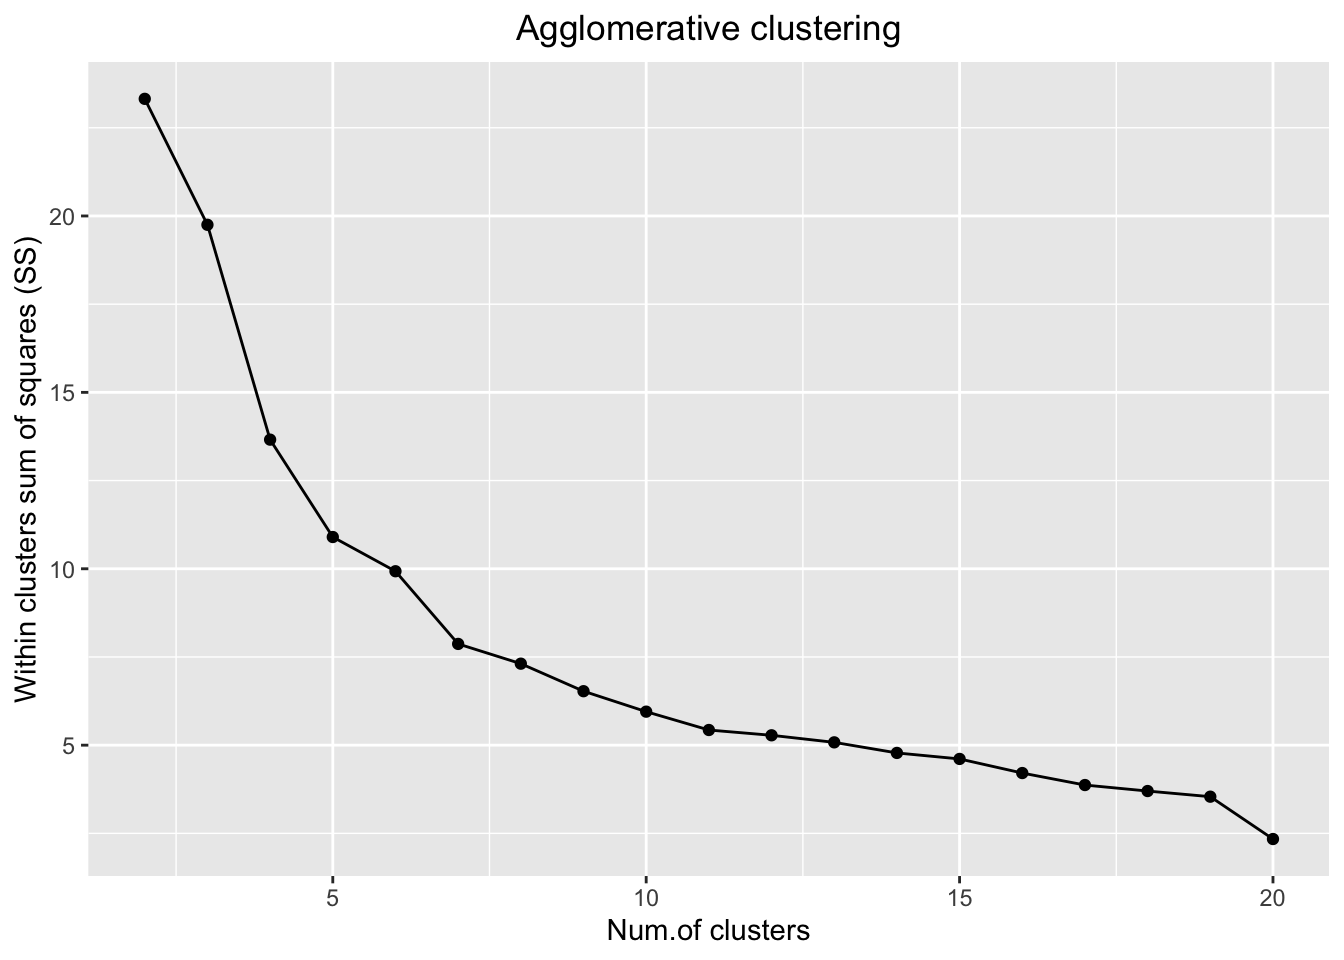
\includegraphics{Albacore_synthesis_b_files/figure-latex/Cluster Selection - Agglomerative-1.pdf}

\begin{Shaded}
\begin{Highlighting}[]
\DocumentationTok{\#\# Silhouette}
\CommentTok{\#When it comes to silhouette assessment, the rule is you should choose the number that maximizes the }
\CommentTok{\#silhouette coefficient because you want clusters that are distinctive (far) enough to be considered separate.}

\CommentTok{\# Agglomerative}
\FunctionTok{ggplot}\NormalTok{(}\AttributeTok{data =} \FunctionTok{data.frame}\NormalTok{(}\FunctionTok{t}\NormalTok{(}\FunctionTok{cstats.table}\NormalTok{(prob.gower.dist, prob.aggl.clustc, }\DecValTok{20}\NormalTok{))), }
       \FunctionTok{aes}\NormalTok{(}\AttributeTok{x=}\NormalTok{cluster.number, }\AttributeTok{y=}\NormalTok{avg.silwidth)) }\SpecialCharTok{+} 
  \FunctionTok{geom\_point}\NormalTok{()}\SpecialCharTok{+}
  \FunctionTok{geom\_line}\NormalTok{()}\SpecialCharTok{+}
  \FunctionTok{ggtitle}\NormalTok{(}\StringTok{"Agglomerative clustering"}\NormalTok{) }\SpecialCharTok{+}
  \FunctionTok{labs}\NormalTok{(}\AttributeTok{x =} \StringTok{"Num.of clusters"}\NormalTok{, }\AttributeTok{y =} \StringTok{"Average silhouette width"}\NormalTok{) }\SpecialCharTok{+}
  \FunctionTok{theme}\NormalTok{(}\AttributeTok{plot.title =} \FunctionTok{element\_text}\NormalTok{(}\AttributeTok{hjust =} \FloatTok{0.5}\NormalTok{))}
\end{Highlighting}
\end{Shaded}

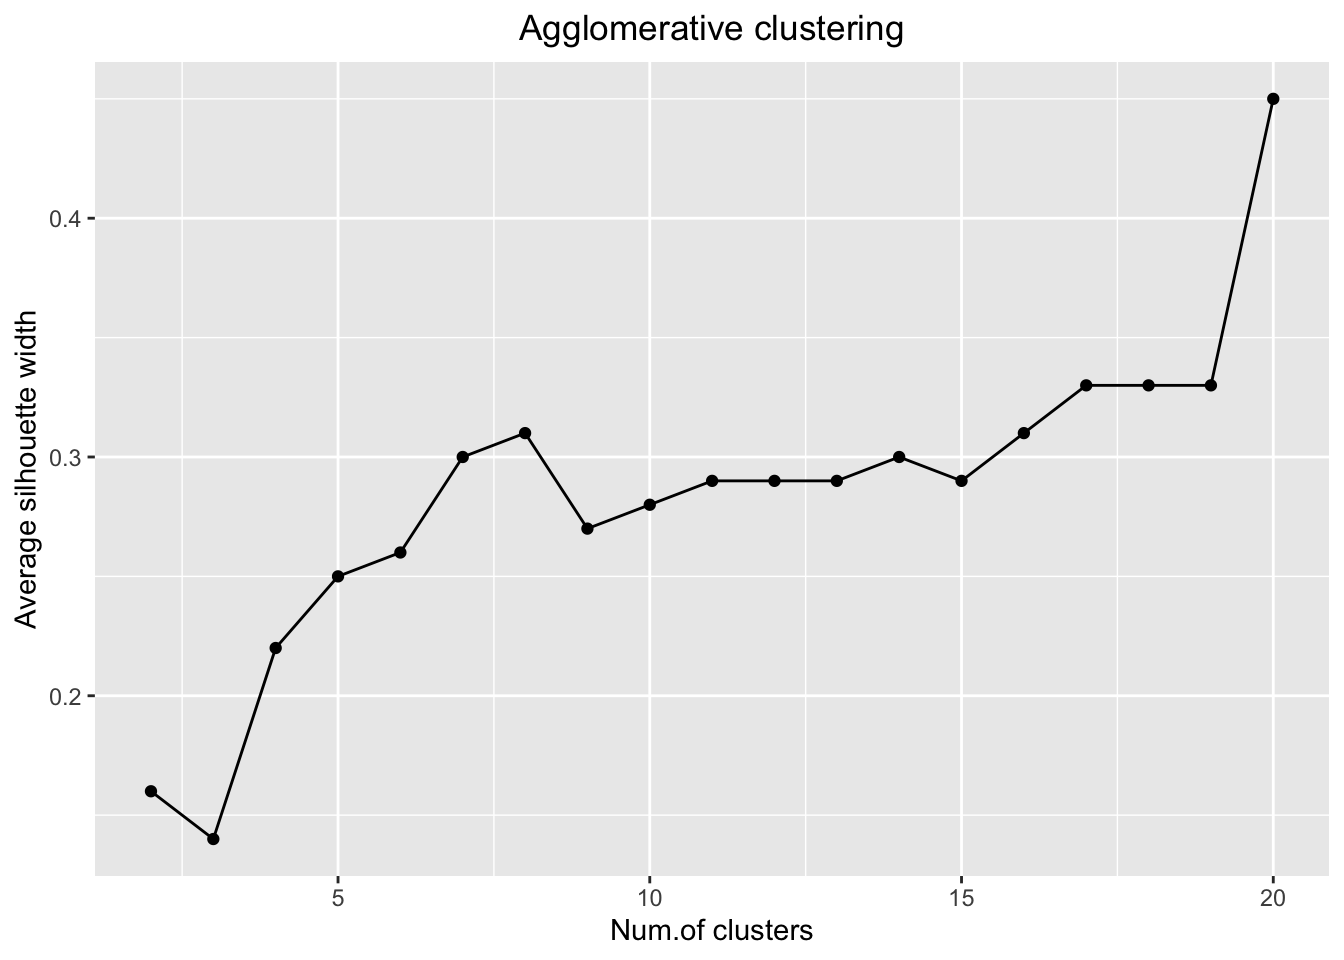
\includegraphics{Albacore_synthesis_b_files/figure-latex/Cluster Selection - Agglomerative-2.pdf}

\textbf{Note} Divisive -- for visualising cluster number selection.

\begin{itemize}
\item
  Elbow method (20/03/2021) using habitat use + gregarious (binary) +
  life stage without refuge use inflection at 7
\item
  Silhouette (20/03/2021) using habitat use + gregarious (binary) + life
  stage without refuge use inflection at 7
\end{itemize}

\begin{Shaded}
\begin{Highlighting}[]
\DocumentationTok{\#\#\# Using "Elbow" and "Silhouette" methods to identify the best number of clusters}

\CommentTok{\# Elbow method}

\CommentTok{\# Agglomerative clustering,provides a more ambiguous picture}
\FunctionTok{ggplot}\NormalTok{(}\AttributeTok{data =} \FunctionTok{data.frame}\NormalTok{(}\FunctionTok{t}\NormalTok{(}\FunctionTok{cstats.table}\NormalTok{(prob.gower.dist, prob.divisive.clust, }\DecValTok{20}\NormalTok{))), }
       \FunctionTok{aes}\NormalTok{(}\AttributeTok{x=}\NormalTok{cluster.number, }\AttributeTok{y=}\NormalTok{within.cluster.ss)) }\SpecialCharTok{+} 
  \FunctionTok{geom\_point}\NormalTok{()}\SpecialCharTok{+}
  \FunctionTok{geom\_line}\NormalTok{()}\SpecialCharTok{+}
  \FunctionTok{ggtitle}\NormalTok{(}\StringTok{"Divisive clustering"}\NormalTok{) }\SpecialCharTok{+}
  \FunctionTok{labs}\NormalTok{(}\AttributeTok{x =} \StringTok{"Num.of clusters"}\NormalTok{, }\AttributeTok{y =} \StringTok{"Within clusters sum of squares (SS)"}\NormalTok{) }\SpecialCharTok{+}
  \FunctionTok{theme}\NormalTok{(}\AttributeTok{plot.title =} \FunctionTok{element\_text}\NormalTok{(}\AttributeTok{hjust =} \FloatTok{0.5}\NormalTok{))}
\end{Highlighting}
\end{Shaded}

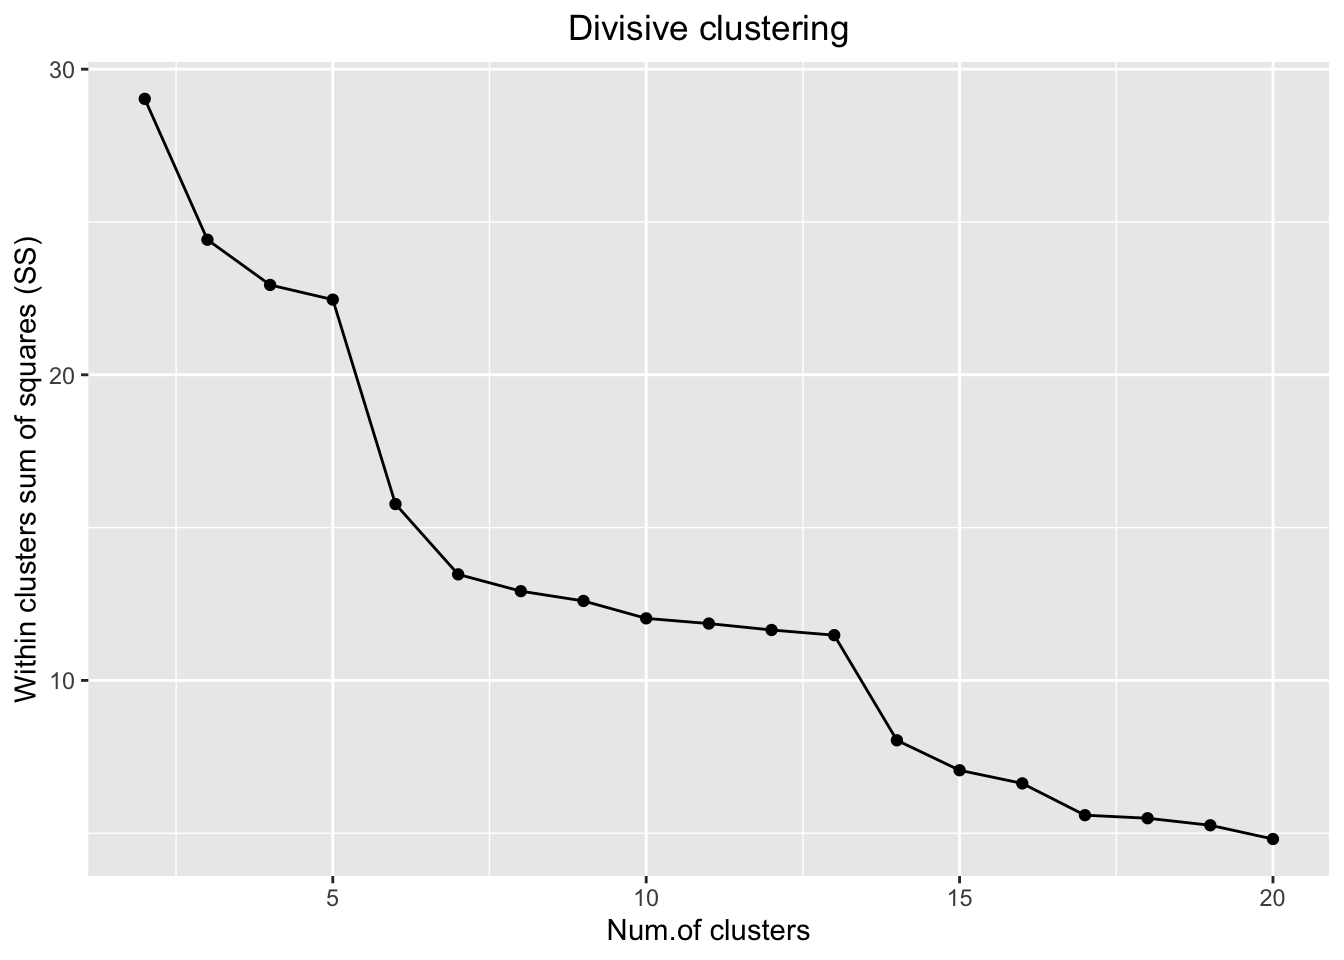
\includegraphics{Albacore_synthesis_b_files/figure-latex/Cluster Selection - Divisive-1.pdf}

\begin{Shaded}
\begin{Highlighting}[]
\DocumentationTok{\#\# Silhouette}
\CommentTok{\#When it comes to silhouette assessment, the rule is you should choose the number that maximizes the }
\CommentTok{\#silhouette coefficient because you want clusters that are distinctive (far) enough to be considered separate.}

\CommentTok{\# Agglomerative}
\FunctionTok{ggplot}\NormalTok{(}\AttributeTok{data =} \FunctionTok{data.frame}\NormalTok{(}\FunctionTok{t}\NormalTok{(}\FunctionTok{cstats.table}\NormalTok{(prob.gower.dist, prob.divisive.clust, }\DecValTok{20}\NormalTok{))), }
       \FunctionTok{aes}\NormalTok{(}\AttributeTok{x=}\NormalTok{cluster.number, }\AttributeTok{y=}\NormalTok{avg.silwidth)) }\SpecialCharTok{+} 
  \FunctionTok{geom\_point}\NormalTok{()}\SpecialCharTok{+}
  \FunctionTok{geom\_line}\NormalTok{()}\SpecialCharTok{+}
  \FunctionTok{ggtitle}\NormalTok{(}\StringTok{"Divisive clustering"}\NormalTok{) }\SpecialCharTok{+}
  \FunctionTok{labs}\NormalTok{(}\AttributeTok{x =} \StringTok{"Num.of clusters"}\NormalTok{, }\AttributeTok{y =} \StringTok{"Average silhouette width"}\NormalTok{) }\SpecialCharTok{+}
  \FunctionTok{theme}\NormalTok{(}\AttributeTok{plot.title =} \FunctionTok{element\_text}\NormalTok{(}\AttributeTok{hjust =} \FloatTok{0.5}\NormalTok{))}
\end{Highlighting}
\end{Shaded}

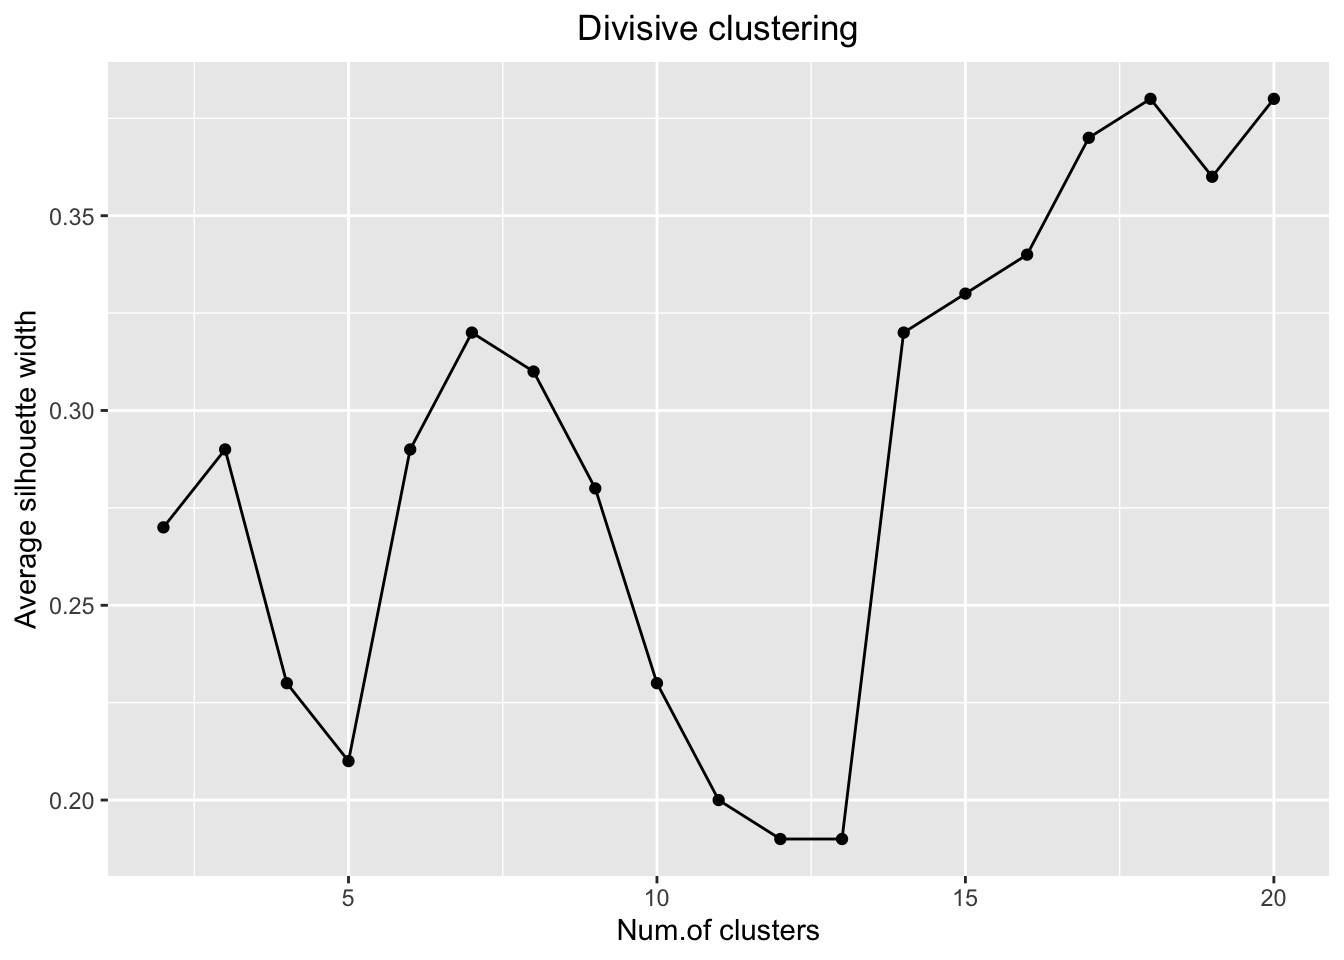
\includegraphics{Albacore_synthesis_b_files/figure-latex/Cluster Selection - Divisive-2.pdf}

\hypertarget{probable-divisive-k-7-excl.-refuge-use}{%
\subsection{PROBABLE Divisive k = 7, excl. refuge
use}\label{probable-divisive-k-7-excl.-refuge-use}}

\hypertarget{cluster-dendrograms}{%
\subsubsection{Cluster Dendrograms ---}\label{cluster-dendrograms}}

Going to use k = 6 for the probable life stage traits

\textbf{Horizontal dendrogram}

\begin{Shaded}
\begin{Highlighting}[]
\CommentTok{\#Using agglomerative hierarchical clustering, k = 8}
\NormalTok{prob.dendro }\OtherTok{\textless{}{-}} \FunctionTok{as.dendrogram}\NormalTok{(prob.divisive.clust) }\CommentTok{\#156 species}
\NormalTok{PNW.pal7 }\OtherTok{\textless{}{-}} \FunctionTok{pnw\_palette}\NormalTok{(}\DecValTok{7}\NormalTok{, }\AttributeTok{name =} \StringTok{"Bay"}\NormalTok{, }\AttributeTok{type =} \StringTok{"continuous"}\NormalTok{)}
\DocumentationTok{\#\#\#Horizontal dendrogram {-} Probable traits}

\CommentTok{\#Horizontal cluster illustration version}
\NormalTok{prob.dendro.col }\OtherTok{\textless{}{-}}\NormalTok{ prob.dendro }\SpecialCharTok{\%\textgreater{}\%}
  \FunctionTok{set}\NormalTok{(}\StringTok{"branches\_k\_color"}\NormalTok{, }\AttributeTok{k =} \DecValTok{7}\NormalTok{, }\AttributeTok{value =}\NormalTok{ PNW.pal7) }\SpecialCharTok{\%\textgreater{}\%}
  \FunctionTok{set}\NormalTok{(}\StringTok{"branches\_lwd"}\NormalTok{, }\FloatTok{0.8}\NormalTok{) }\SpecialCharTok{\%\textgreater{}\%}
  \FunctionTok{set}\NormalTok{(}\StringTok{"labels"}\NormalTok{, probable\_species) }\SpecialCharTok{\%\textgreater{}\%} \CommentTok{\#NOT VERY LEGIBLE...}
  \FunctionTok{set}\NormalTok{(}\StringTok{"labels\_colors"}\NormalTok{, }
      \AttributeTok{value =} \FunctionTok{c}\NormalTok{(}\StringTok{"darkslategray"}\NormalTok{)) }\SpecialCharTok{\%\textgreater{}\%} 
  \FunctionTok{set}\NormalTok{(}\StringTok{"labels\_cex"}\NormalTok{, }\FloatTok{0.5}\NormalTok{)}
\NormalTok{prob.ggd1 }\OtherTok{\textless{}{-}} \FunctionTok{as.ggdend}\NormalTok{(prob.dendro.col)}
\NormalTok{prob.dendro.graph }\OtherTok{\textless{}{-}} \FunctionTok{ggplot}\NormalTok{(prob.ggd1, }\AttributeTok{theme =} \FunctionTok{theme\_minimal}\NormalTok{()) }\SpecialCharTok{+}
  \FunctionTok{labs}\NormalTok{(}\AttributeTok{x =} \StringTok{"Num. observations"}\NormalTok{, }\AttributeTok{y =} \StringTok{"Height"}\NormalTok{, }\AttributeTok{title =} \StringTok{"Dendrogram, k = 6"}\NormalTok{)}
\NormalTok{prob.dendro.graph}
\end{Highlighting}
\end{Shaded}

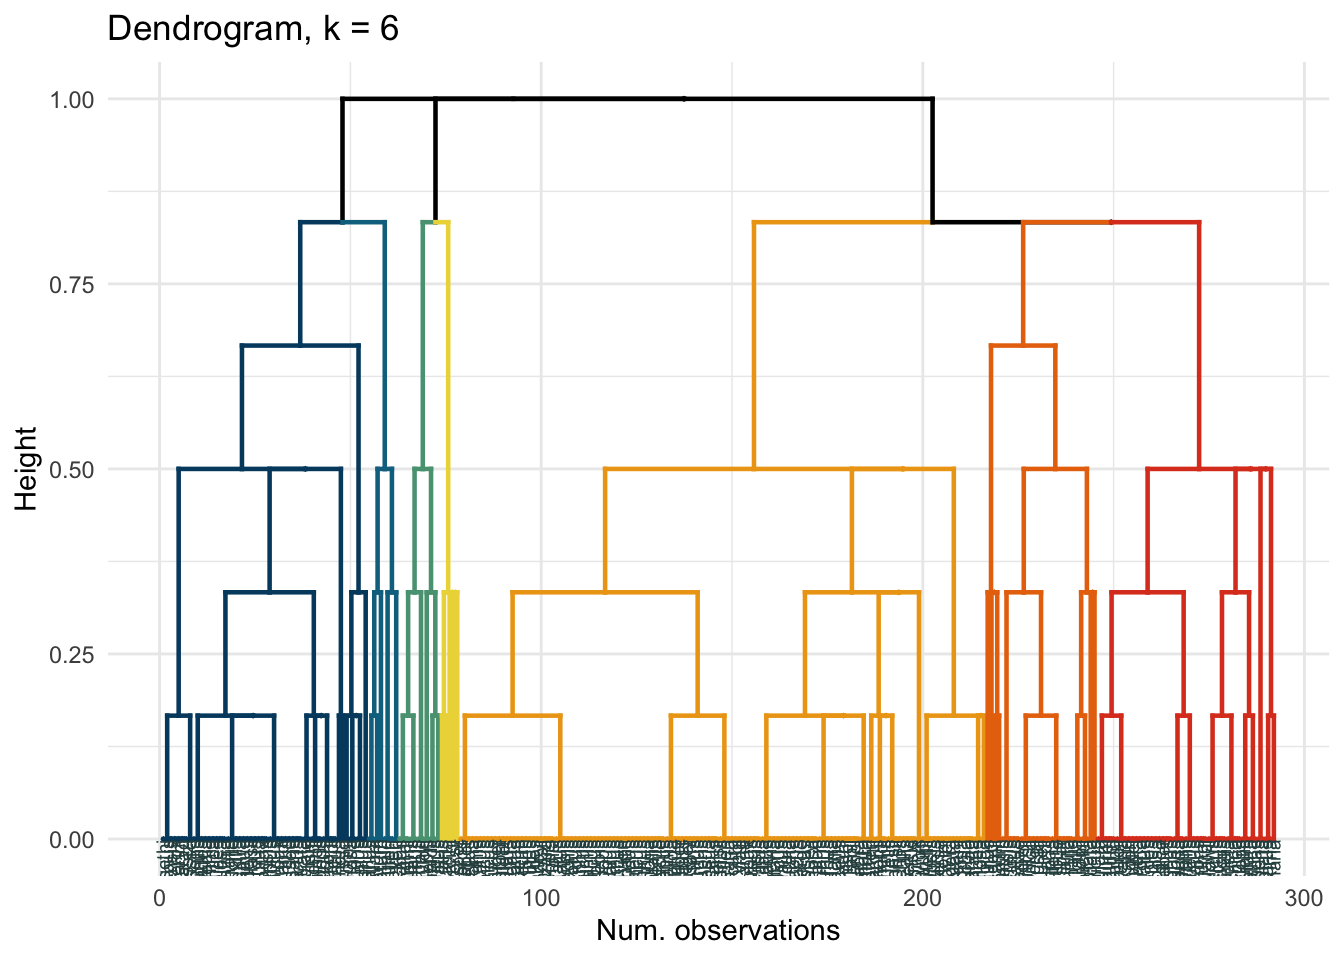
\includegraphics{Albacore_synthesis_b_files/figure-latex/Horizontal dendrogram-1.pdf}

\begin{Shaded}
\begin{Highlighting}[]
\FunctionTok{ggsave}\NormalTok{(}\FunctionTok{here}\NormalTok{(}\StringTok{\textquotesingle{}outputs\_figures/clusters/probable\_divis\_simple/prob.dendro.horz.k7.png\textquotesingle{}}\NormalTok{), }\AttributeTok{plot=}\NormalTok{prob.dendro.graph, }\AttributeTok{width=}\DecValTok{8}\NormalTok{, }\AttributeTok{height=}\DecValTok{8}\NormalTok{, }\AttributeTok{dpi=}\DecValTok{300}\NormalTok{)}
\end{Highlighting}
\end{Shaded}

\textbf{Radial dendrogram}

\begin{Shaded}
\begin{Highlighting}[]
\CommentTok{\# Radial plot looks less cluttered (and cooler)}
\NormalTok{prob.dendro.rad }\OtherTok{\textless{}{-}} \FunctionTok{ggplot}\NormalTok{(prob.ggd1, }\AttributeTok{labels =} \ConstantTok{FALSE}\NormalTok{) }\SpecialCharTok{+} 
  \FunctionTok{scale\_y\_reverse}\NormalTok{(}\AttributeTok{expand =} \FunctionTok{c}\NormalTok{(}\FloatTok{0.2}\NormalTok{, }\DecValTok{0}\NormalTok{)) }\SpecialCharTok{+}
  \FunctionTok{coord\_polar}\NormalTok{(}\AttributeTok{theta=}\StringTok{"x"}\NormalTok{)}
\NormalTok{prob.dendro.rad }
\end{Highlighting}
\end{Shaded}

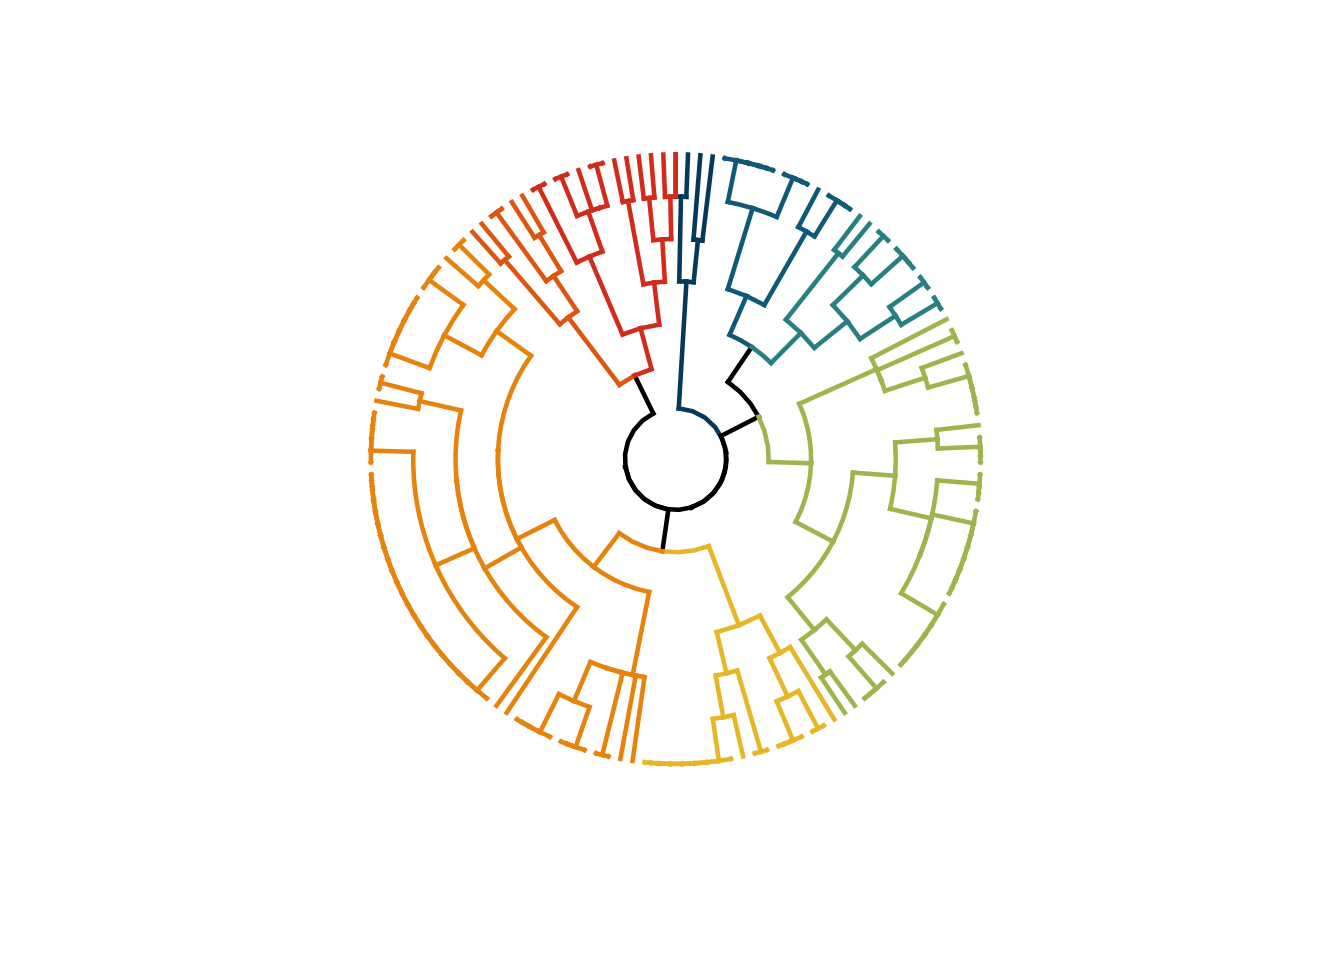
\includegraphics{Albacore_synthesis_b_files/figure-latex/Radial dendrogram-1.pdf}

\begin{Shaded}
\begin{Highlighting}[]
\CommentTok{\#No labels on this one, labels were too cluttered/problems}
\CommentTok{\#Save radial dendrogram for chat}

\FunctionTok{ggsave}\NormalTok{(}\FunctionTok{here}\NormalTok{(}\StringTok{\textquotesingle{}outputs\_figures/clusters/probable\_divis\_simple/prob.dendro.rad.k7.png\textquotesingle{}}\NormalTok{), }\AttributeTok{plot=}\NormalTok{prob.dendro.rad, }\AttributeTok{width=}\DecValTok{8}\NormalTok{, }\AttributeTok{height=}\DecValTok{8}\NormalTok{, }\AttributeTok{dpi=}\DecValTok{300}\NormalTok{)}
\end{Highlighting}
\end{Shaded}

\textbf{Vertical dendrogram}

Similar to
\url{https://stackoverflow.com/questions/38034663/rotate-labels-for-ggplot-dendrogram}

\begin{Shaded}
\begin{Highlighting}[]
\CommentTok{\# This is a different way to compute hierarchical clustering and cut the tree}
\CommentTok{\#clus \textless{}{-} hcut(mydist, k = 6, hc\_func = \textquotesingle{}hclust\textquotesingle{}, hc\_method = \textquotesingle{}ward.D2\textquotesingle{}, graph = FALSE, isdiss = TRUE)}

\CommentTok{\#Below is problematic0}
\CommentTok{\#labels(dend) \textless{}{-} paste0(paste0(rep(\textquotesingle{}\textquotesingle{}, 3), collapse = \textquotesingle{}\textquotesingle{}), speciesO)}
\CommentTok{\#dend \textless{}{-} sort(dend, decreasing = FALSE)}
\CommentTok{\#View(labels(dend))}

\CommentTok{\#Creating df for the dend labels so that we can accurately line them up with the species}
\NormalTok{dendlabs }\OtherTok{\textless{}{-}} \FunctionTok{labels}\NormalTok{(prob.dendro) }\CommentTok{\#Need to create strings of labels to manipulate}
\NormalTok{dendlabs2 }\OtherTok{\textless{}{-}} \FunctionTok{as.data.frame}\NormalTok{(dendlabs) }\CommentTok{\#turn in df}

\CommentTok{\#Join these data so we can relabel the dendrogram}
\CommentTok{\#Use plyr function because it conserves the row order of the left df, which matters for assigning labels here}

\NormalTok{dfdend }\OtherTok{\textless{}{-}} \FunctionTok{join}\NormalTok{(dendlabs2, prey\_probable)}

\NormalTok{ggd1 }\OtherTok{\textless{}{-}} \FunctionTok{ggplot}\NormalTok{(prob.dendro }\SpecialCharTok{\%\textgreater{}\%}
                 \FunctionTok{set}\NormalTok{(}\StringTok{"branches\_k\_color"}\NormalTok{, }\AttributeTok{k =} \DecValTok{7}\NormalTok{, }\AttributeTok{value =}\NormalTok{ PNW.pal7) }\SpecialCharTok{\%\textgreater{}\%}
                 \FunctionTok{set}\NormalTok{(}\StringTok{"branches\_lwd"}\NormalTok{, }\FloatTok{0.8}\NormalTok{) }\SpecialCharTok{\%\textgreater{}\%}
                 \FunctionTok{set}\NormalTok{(}\StringTok{"labels"}\NormalTok{, dfdend}\SpecialCharTok{$}\NormalTok{prey\_sp) }\SpecialCharTok{\%\textgreater{}\%} \CommentTok{\#NOT VERY LEGIBLE...}
                 \FunctionTok{set}\NormalTok{(}\StringTok{"labels\_colors"}\NormalTok{, }
                     \AttributeTok{value =} \FunctionTok{c}\NormalTok{(}\StringTok{"darkslategray"}\NormalTok{)) }\SpecialCharTok{\%\textgreater{}\%} 
                 \FunctionTok{set}\NormalTok{(}\StringTok{"labels\_cex"}\NormalTok{, }\FloatTok{0.5}\NormalTok{), }
               \AttributeTok{theme =} \FunctionTok{theme\_minimal}\NormalTok{(),}
               \AttributeTok{horiz =} \ConstantTok{TRUE}\NormalTok{)}

\NormalTok{ggd1 }\OtherTok{\textless{}{-}}\NormalTok{ ggd1 }\SpecialCharTok{+} \FunctionTok{theme}\NormalTok{(}\AttributeTok{panel.grid.major =} \FunctionTok{element\_blank}\NormalTok{(),}
                     \AttributeTok{axis.text =} \FunctionTok{element\_blank}\NormalTok{(),}
                     \AttributeTok{axis.title =} \FunctionTok{element\_blank}\NormalTok{())}
\NormalTok{ggd1 }\OtherTok{\textless{}{-}}\NormalTok{ ggd1 }\SpecialCharTok{+} \FunctionTok{ylim}\NormalTok{(}\FunctionTok{max}\NormalTok{(}\FunctionTok{get\_branches\_heights}\NormalTok{(prob.dendro)), }\SpecialCharTok{{-}}\DecValTok{1}\NormalTok{)}
\NormalTok{ggd1}
\end{Highlighting}
\end{Shaded}

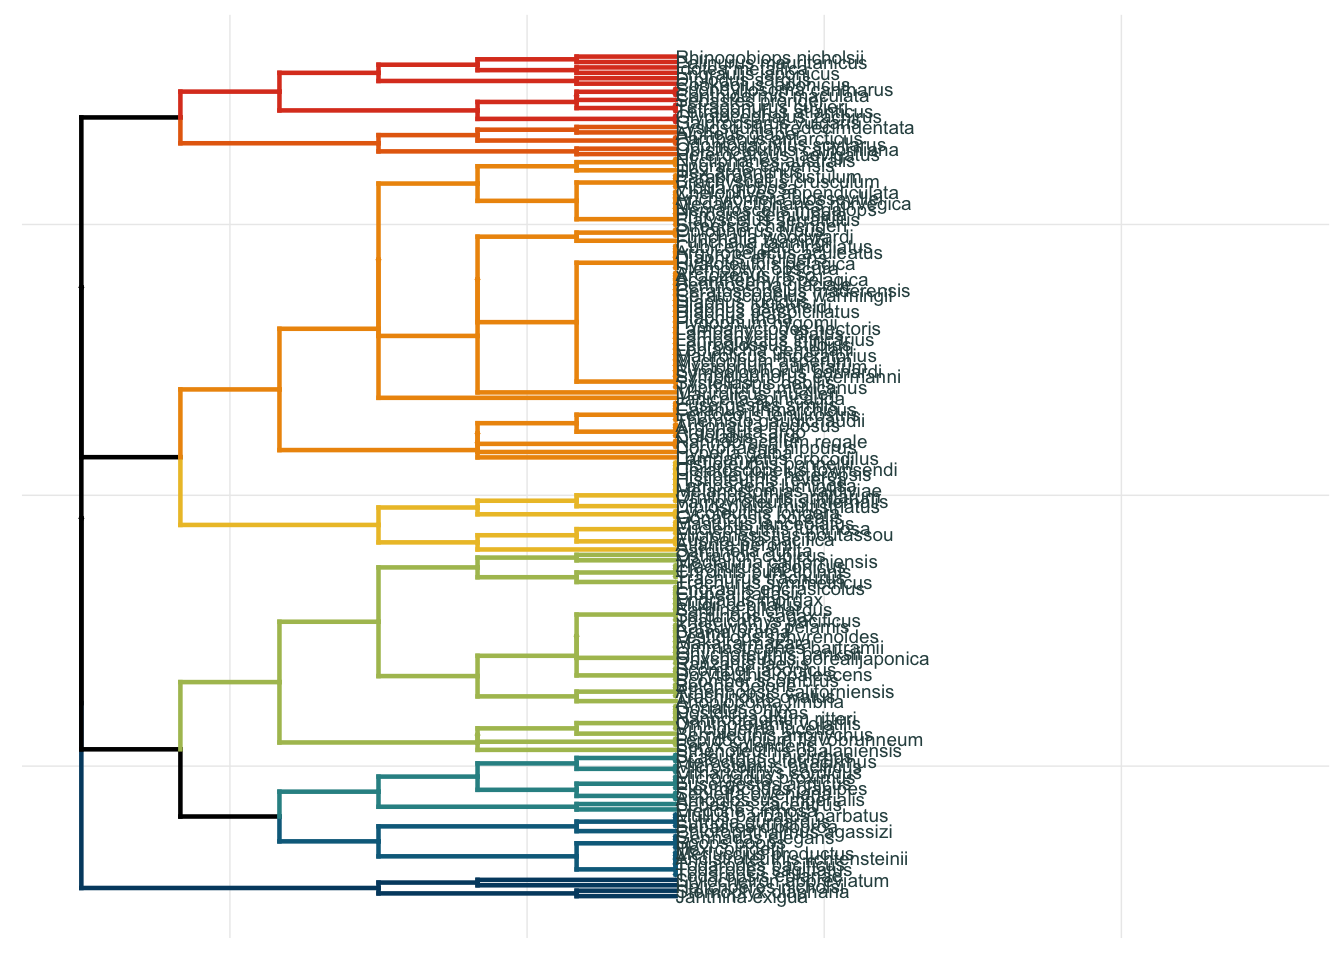
\includegraphics{Albacore_synthesis_b_files/figure-latex/Vertical dendrogram-1.pdf}

\begin{Shaded}
\begin{Highlighting}[]
\FunctionTok{ggsave}\NormalTok{(}\FunctionTok{here}\NormalTok{(}\StringTok{\textquotesingle{}outputs\_figures/clusters/probable\_divis\_simple/prob.dendro.vertlabs.k7.pdf\textquotesingle{}}\NormalTok{), }\AttributeTok{plot=}\NormalTok{ggd1, }\AttributeTok{width=}\DecValTok{5}\NormalTok{, }\AttributeTok{height=}\DecValTok{20}\NormalTok{, }\AttributeTok{dpi=}\DecValTok{300}\NormalTok{)}

\CommentTok{\#With labels removed!!!}

\NormalTok{prob.dendro.vert }\OtherTok{\textless{}{-}} \FunctionTok{ggplot}\NormalTok{(prob.ggd1, }\AttributeTok{horiz =} \ConstantTok{TRUE}\NormalTok{, }\AttributeTok{labels =} \ConstantTok{FALSE}\NormalTok{) }\SpecialCharTok{+} 
  \FunctionTok{scale\_y\_reverse}\NormalTok{(}\AttributeTok{expand =} \FunctionTok{c}\NormalTok{(}\FloatTok{0.2}\NormalTok{, }\DecValTok{0}\NormalTok{)) }\CommentTok{\#+}
\CommentTok{\#coord\_polar(theta="x")}
\NormalTok{prob.dendro.vert }
\end{Highlighting}
\end{Shaded}

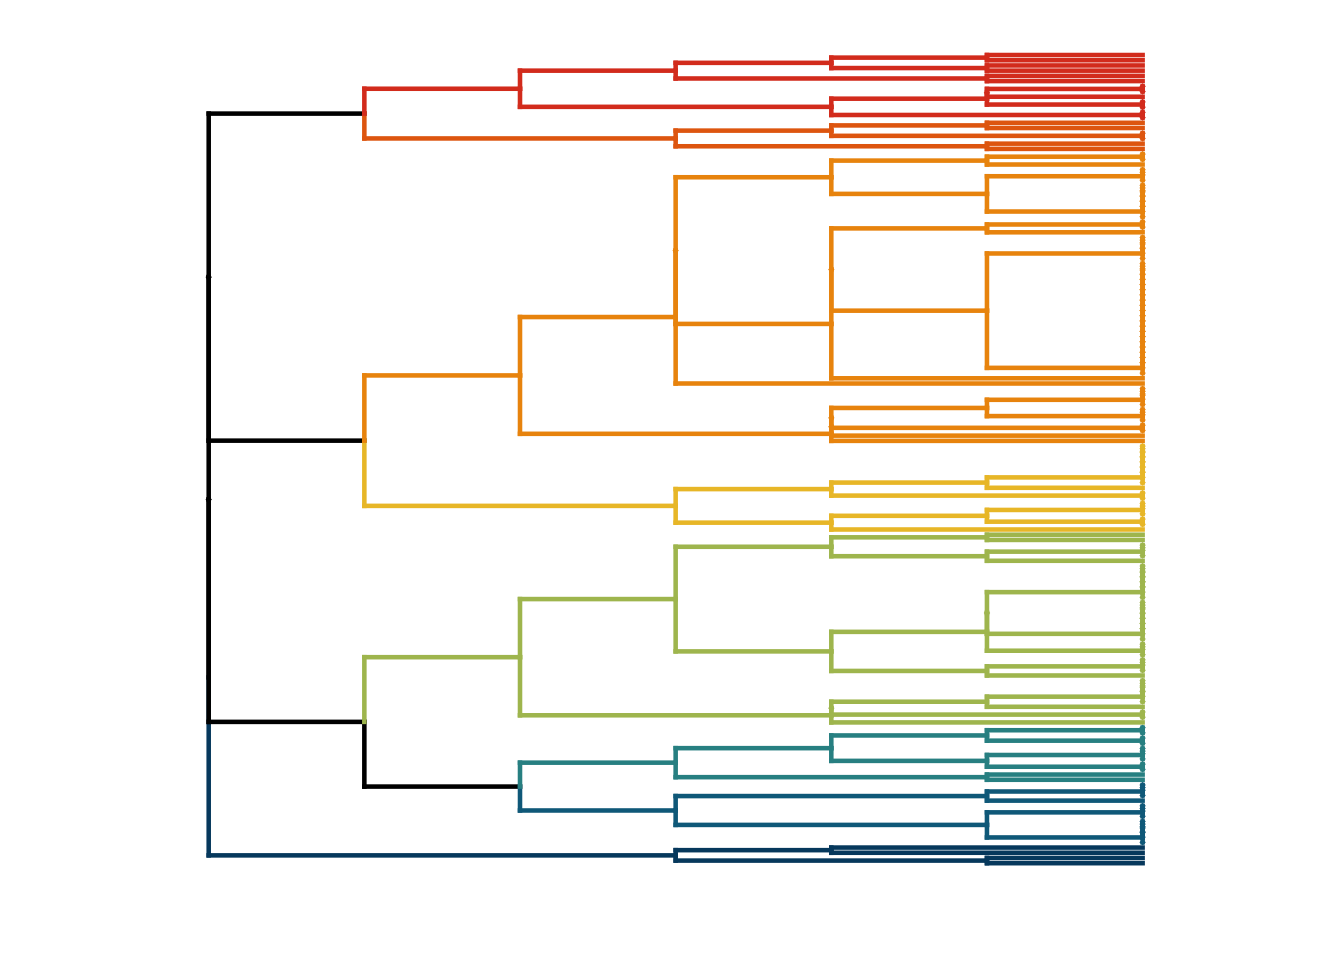
\includegraphics{Albacore_synthesis_b_files/figure-latex/Vertical dendrogram-2.pdf}

\begin{Shaded}
\begin{Highlighting}[]
\CommentTok{\#Export as .png}
\FunctionTok{ggsave}\NormalTok{(}\FunctionTok{here}\NormalTok{(}\StringTok{\textquotesingle{}outputs\_figures/clusters/probable\_divis\_simple/prob.dendro.vert2.k7.png\textquotesingle{}}\NormalTok{), }\AttributeTok{plot=}\NormalTok{prob.dendro.vert, }\AttributeTok{width=}\DecValTok{5}\NormalTok{, }\AttributeTok{height=}\DecValTok{12}\NormalTok{, }\AttributeTok{dpi=}\DecValTok{300}\NormalTok{)}
\end{Highlighting}
\end{Shaded}

\hypertarget{albacore-cluster-heatmap--}{%
\subsubsection{Albacore Cluster Heatmap
----}\label{albacore-cluster-heatmap--}}

\begin{Shaded}
\begin{Highlighting}[]
\CommentTok{\#Extract cluster number to trait matrix}
\NormalTok{prob.clust.num }\OtherTok{\textless{}{-}} \FunctionTok{cutree}\NormalTok{(prob.divisive.clust, }\AttributeTok{k =} \DecValTok{7}\NormalTok{)}

\CommentTok{\#we want to bind the original dataset with the cluster numbers such that each species is assigned a cluster}
\CommentTok{\#can use whole data or just traits use to just look at unique species clusters in relation to traits}
\CommentTok{\#alb.cl \textless{}{-} cbind(ctraitsO, alb.clust.num)}
\CommentTok{\#OR}
\NormalTok{prob.prey.cl }\OtherTok{\textless{}{-}} \FunctionTok{cbind}\NormalTok{(prey\_probable, prob.clust.num)}

\CommentTok{\#View(prob.prey.cl)}

\CommentTok{\#write.csv(prob.prey.cl, here("data/output\_data/prob.prey.clusternum\_habgreg.divis.k8.csv"))}
\FunctionTok{write.csv}\NormalTok{(prob.prey.cl, }\FunctionTok{here}\NormalTok{(}\StringTok{"outputs\_figures/clusters/probable\_divis\_simple/prob.prey.clusternum\_habgreg.divis.k7.csv"}\NormalTok{))}
\end{Highlighting}
\end{Shaded}

\begin{Shaded}
\begin{Highlighting}[]
\CommentTok{\# Time for the heatmap}
\CommentTok{\# the 1st step here is to have 1 variable per row}
\CommentTok{\# factors have to be converted to characters in order not to be dropped}

\CommentTok{\#Note plyr can mess with this!!}
\FunctionTok{detach}\NormalTok{(}\StringTok{"package:plyr"}\NormalTok{, }\AttributeTok{unload=}\ConstantTok{TRUE}\NormalTok{)}

\CommentTok{\#Create dfs for graphs}
\NormalTok{prob.clust.long }\OtherTok{=}\NormalTok{ prob.prey.cl }\SpecialCharTok{\%\textgreater{}\%}
\NormalTok{  dplyr}\SpecialCharTok{::}\FunctionTok{select}\NormalTok{(prey\_sp, life\_stage}\SpecialCharTok{:}\NormalTok{season\_cat, }\StringTok{\textasciigrave{}}\AttributeTok{gregarious}\StringTok{\textasciigrave{}}\NormalTok{, }\StringTok{\textasciigrave{}}\AttributeTok{prob.clust.num}\StringTok{\textasciigrave{}}\NormalTok{, }\SpecialCharTok{{-}}\NormalTok{refuge\_cat) }\SpecialCharTok{\%\textgreater{}\%} \CommentTok{\#maxFO:maxM, }
\NormalTok{  reshape2}\SpecialCharTok{::}\FunctionTok{melt}\NormalTok{(}\AttributeTok{id.vars =} \FunctionTok{c}\NormalTok{(}\StringTok{"prey\_sp"}\NormalTok{, }\StringTok{"prob.clust.num"}\NormalTok{), }\AttributeTok{variable.name =} \StringTok{"trait"}\NormalTok{, }\AttributeTok{value.name =} \StringTok{"level"}\NormalTok{) }\SpecialCharTok{\%\textgreater{}\%}
  \FunctionTok{group\_by}\NormalTok{(prob.clust.num, trait, level) }\SpecialCharTok{\%\textgreater{}\%}
  \FunctionTok{mutate}\NormalTok{(}\AttributeTok{count =} \FunctionTok{n\_distinct}\NormalTok{(prey\_sp)) }\SpecialCharTok{\%\textgreater{}\%}
  \FunctionTok{distinct}\NormalTok{(prob.clust.num, trait, level, count) }\SpecialCharTok{\%\textgreater{}\%} \CommentTok{\#, percent}
  \FunctionTok{group\_by}\NormalTok{(prob.clust.num, trait) }\SpecialCharTok{\%\textgreater{}\%}
  \FunctionTok{mutate}\NormalTok{(}\AttributeTok{percent =}\NormalTok{ count }\SpecialCharTok{/} \FunctionTok{sum}\NormalTok{(count)}\SpecialCharTok{*}\DecValTok{100}\NormalTok{) }\SpecialCharTok{\%\textgreater{}\%}
  \FunctionTok{arrange}\NormalTok{(prob.clust.num)}

\CommentTok{\#str(prob.clust.long)}

\CommentTok{\#heatmap.c will be suitable in case you want to go for absolute counts {-} but it doesn\textquotesingle{}t tell much to my taste}
\CommentTok{\#problem below involves the values of our data being ordinal, therefore they are not unique}
\FunctionTok{levels}\NormalTok{(prob.clust.long}\SpecialCharTok{$}\NormalTok{trait)}
\end{Highlighting}
\end{Shaded}

\begin{verbatim}
## [1] "life_stage"       "vert_habitat"     "horz_habitat"     "diel_migrant_cat"
## [5] "season_cat"       "gregarious"
\end{verbatim}

\begin{Shaded}
\begin{Highlighting}[]
\CommentTok{\#Our data above comes truncated, you would need to truncate the data and re{-}label clusters depending on which dfs you melt/merge/reshape.}
\CommentTok{\#Example: View(alb.cust.long.q[96:nrow(alb.cust.long.q),])}
\NormalTok{heatmap.c }\OtherTok{\textless{}{-}} \FunctionTok{ggplot}\NormalTok{(prob.clust.long, }\FunctionTok{aes}\NormalTok{(}\AttributeTok{x =} \FunctionTok{factor}\NormalTok{(prob.clust.num), }\AttributeTok{y =}\NormalTok{ level)) }\SpecialCharTok{+}
  \FunctionTok{geom\_tile}\NormalTok{(}\FunctionTok{aes}\NormalTok{(}\AttributeTok{fill =}\NormalTok{ count))}\SpecialCharTok{+}
  \FunctionTok{labs}\NormalTok{(}\AttributeTok{title =} \StringTok{"Distribution of characteristics across clusters"}\NormalTok{, }\AttributeTok{x =} \StringTok{"Cluster number"}\NormalTok{, }\AttributeTok{y =} \ConstantTok{NULL}\NormalTok{) }\SpecialCharTok{+}
  \FunctionTok{scale\_fill\_viridis}\NormalTok{(}\AttributeTok{option=}\StringTok{"magma"}\NormalTok{, }\AttributeTok{begin =} \FloatTok{0.2}\NormalTok{, }\AttributeTok{end =} \FloatTok{0.95}\NormalTok{)}\SpecialCharTok{+}
  \FunctionTok{facet\_grid}\NormalTok{(trait}\SpecialCharTok{\textasciitilde{}}\NormalTok{. , }\AttributeTok{scales=}\StringTok{"free\_y"}\NormalTok{)}
\NormalTok{heatmap.c}
\end{Highlighting}
\end{Shaded}

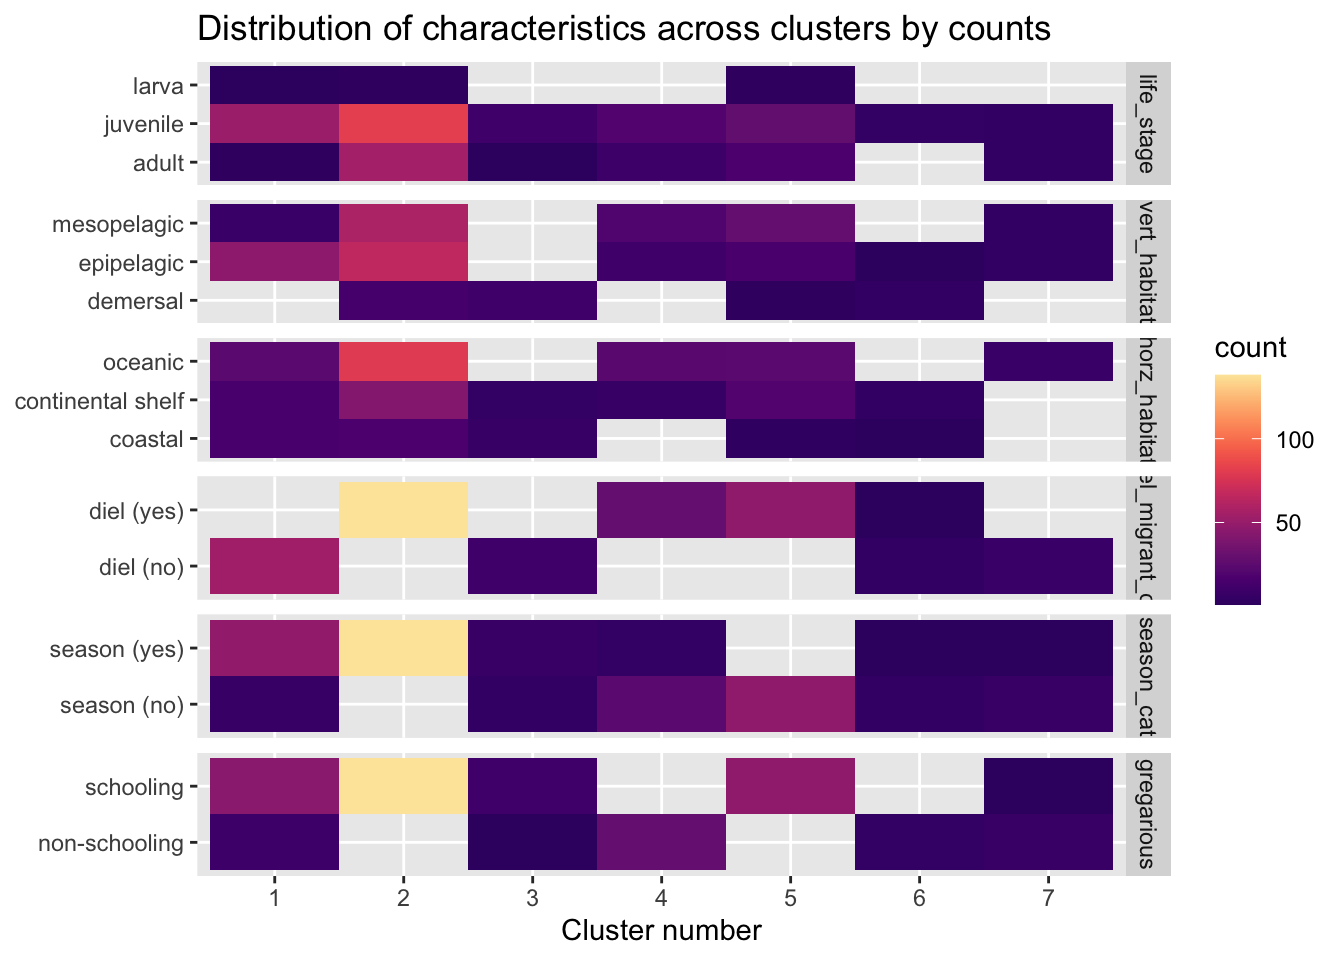
\includegraphics{Albacore_synthesis_b_files/figure-latex/Cluster heatmap-1.pdf}

\begin{Shaded}
\begin{Highlighting}[]
\FunctionTok{ggsave}\NormalTok{(}\FunctionTok{here}\NormalTok{(}\StringTok{\textquotesingle{}outputs\_figures/clusters/probable\_divis\_simple/prob.dendro.heatcounts.divis.k7.life.pdf\textquotesingle{}}\NormalTok{), }\AttributeTok{plot=}\NormalTok{heatmap.c, }\AttributeTok{width=}\DecValTok{8}\NormalTok{, }\AttributeTok{height=}\DecValTok{12}\NormalTok{, }\AttributeTok{dpi=}\DecValTok{300}\NormalTok{)}


\NormalTok{heatmap.p }\OtherTok{\textless{}{-}} \FunctionTok{ggplot}\NormalTok{(prob.clust.long, }\FunctionTok{aes}\NormalTok{(}\AttributeTok{x =} \FunctionTok{factor}\NormalTok{(prob.clust.num), }\AttributeTok{y =} \FunctionTok{factor}\NormalTok{(level, }\AttributeTok{ordered =}\NormalTok{ T))) }\SpecialCharTok{+}
  \FunctionTok{geom\_tile}\NormalTok{(}\FunctionTok{aes}\NormalTok{(}\AttributeTok{fill =}\NormalTok{ percent), }\AttributeTok{alpha =} \FloatTok{0.85}\NormalTok{)}\SpecialCharTok{+}
  \FunctionTok{labs}\NormalTok{(}\AttributeTok{title =} \StringTok{"Distribution of characteristics across clusters"}\NormalTok{, }\AttributeTok{x =} \StringTok{"Cluster number"}\NormalTok{, }\AttributeTok{y =} \ConstantTok{NULL}\NormalTok{) }\SpecialCharTok{+}
  \CommentTok{\#scale\_fill\_gradient2(low = "darkslategray1", mid = "yellow", high = "turquoise4") +}
  \FunctionTok{scale\_fill\_viridis}\NormalTok{(}\AttributeTok{option=}\StringTok{"magma"}\NormalTok{, }\AttributeTok{begin =} \FloatTok{0.2}\NormalTok{, }\AttributeTok{end =} \FloatTok{0.95}\NormalTok{)}\SpecialCharTok{+}
  \FunctionTok{facet\_grid}\NormalTok{(trait}\SpecialCharTok{\textasciitilde{}}\NormalTok{., }\AttributeTok{scales=}\StringTok{"free\_y"}\NormalTok{)}
\NormalTok{heatmap.p}
\end{Highlighting}
\end{Shaded}

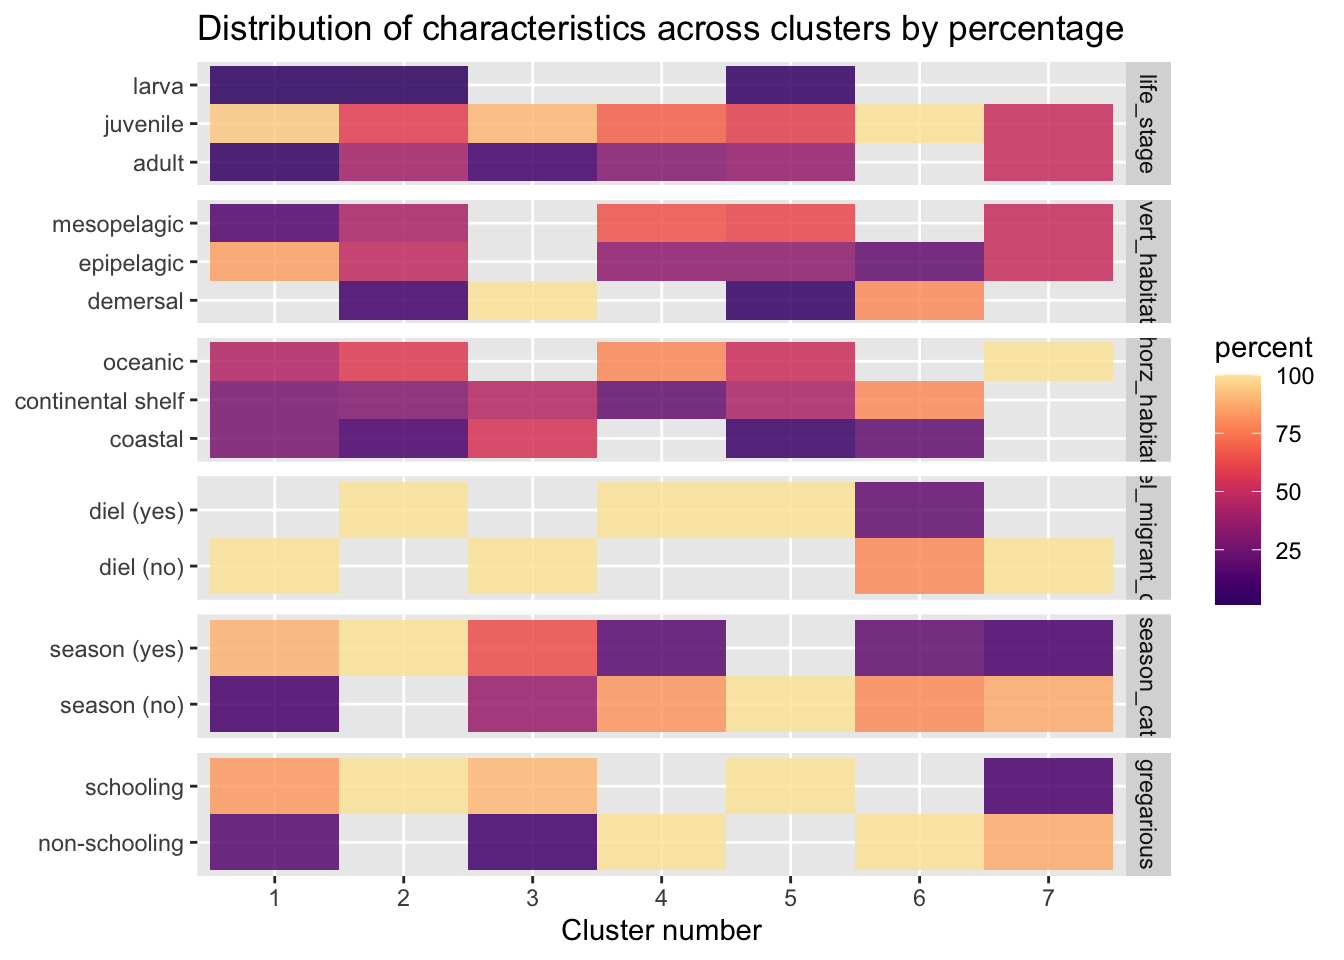
\includegraphics{Albacore_synthesis_b_files/figure-latex/Cluster heatmap-2.pdf}

\begin{Shaded}
\begin{Highlighting}[]
\FunctionTok{ggsave}\NormalTok{(}\FunctionTok{here}\NormalTok{(}\StringTok{\textquotesingle{}outputs\_figures/clusters/probable\_divis\_simple/prob.dendro.heatpercent.divis.k7.life.pdf\textquotesingle{}}\NormalTok{), }\AttributeTok{plot=}\NormalTok{heatmap.p, }\AttributeTok{width=}\DecValTok{8}\NormalTok{, }\AttributeTok{height=}\DecValTok{12}\NormalTok{, }\AttributeTok{dpi=}\DecValTok{300}\NormalTok{)}
\end{Highlighting}
\end{Shaded}

\begin{Shaded}
\begin{Highlighting}[]
\FunctionTok{summary}\NormalTok{(}\FunctionTok{as.factor}\NormalTok{(prob.prey.cl}\SpecialCharTok{$}\NormalTok{prob.clust.num))}
\CommentTok{\#clusters  1  2  3  4  5  6  7 }
\CommentTok{\#         31 36 26 21  8 21 13 }
\end{Highlighting}
\end{Shaded}

\hypertarget{nmds-for-checking-on-our-ordination---divisive}{%
\subsection{NMDS for checking on our ordination -
divisive}\label{nmds-for-checking-on-our-ordination---divisive}}

\hypertarget{ordination}{%
\subsubsection{Ordination}\label{ordination}}

\begin{Shaded}
\begin{Highlighting}[]
\DocumentationTok{\#\#\#\# nMDS for dissimilarity}
\NormalTok{trait\_NMDS\_prob }\OtherTok{\textless{}{-}} \FunctionTok{metaMDS}\NormalTok{(prob.gower.dist, }\AttributeTok{trymax =} \DecValTok{1000}\NormalTok{)  }\CommentTok{\#solution after 541 iterations}
\NormalTok{trait\_NMDS\_prob[[}\StringTok{"stress"}\NormalTok{]]  }\CommentTok{\#stress = 0.1477077 \#reasonable}
\end{Highlighting}
\end{Shaded}

\hypertarget{extract-nmds-coordinates-and-associate-with-co-variatesgrouping-factors}{%
\subsubsection{Extract NMDS coordinates and associate with
co-variates/grouping
factors}\label{extract-nmds-coordinates-and-associate-with-co-variatesgrouping-factors}}

\begin{Shaded}
\begin{Highlighting}[]
\CommentTok{\#Extract NMDS coordinates and associate with co{-}variates/grouping factors}

\CommentTok{\#Using the scores function from vegan to extract the site scores and convert to a data.frame}
\NormalTok{data.scores }\OtherTok{\textless{}{-}} \FunctionTok{as.data.frame}\NormalTok{(}\FunctionTok{scores}\NormalTok{(trait\_NMDS\_prob))  }\CommentTok{\#, "species"}

\CommentTok{\#create a column of site names, from the rownames of data.scores}
\NormalTok{data.scores}\SpecialCharTok{$}\NormalTok{points }\OtherTok{\textless{}{-}} \FunctionTok{rownames}\NormalTok{(data.scores)}

\CommentTok{\#bind treatment labels and score values}
\NormalTok{treatment.scores }\OtherTok{\textless{}{-}} \FunctionTok{cbind}\NormalTok{(prob.prey.cl, data.scores)}

\CommentTok{\#Check}
\FunctionTok{str}\NormalTok{(treatment.scores)  }
\CommentTok{\#Awesome}
\end{Highlighting}
\end{Shaded}

\hypertarget{convex-hull-calculations}{%
\subsubsection{Convex hull
calculations}\label{convex-hull-calculations}}

For each ordination and set of grouping variables input to data scores
chunk

\begin{Shaded}
\begin{Highlighting}[]
\CommentTok{\# Taxonomic groups (specific)}
\CommentTok{\#Create convex hulls for the space occupied by each Taxonomic values}
\FunctionTok{unique}\NormalTok{(treatment.scores}\SpecialCharTok{$}\NormalTok{prob.clust.num)}
\FunctionTok{length}\NormalTok{(treatment.scores}\SpecialCharTok{$}\NormalTok{prob.clust.num) }\CommentTok{\#174}

\CommentTok{\#Taxonomic group {-} hull loop}
\NormalTok{clust }\OtherTok{=} \FunctionTok{as.character}\NormalTok{(}\FunctionTok{unique}\NormalTok{(treatment.scores}\SpecialCharTok{$}\NormalTok{prob.clust.num))}
\ControlFlowTok{for}\NormalTok{(i }\ControlFlowTok{in} \DecValTok{1}\SpecialCharTok{:}\FunctionTok{length}\NormalTok{(clust)) \{}
\NormalTok{  temp }\OtherTok{=}\NormalTok{ clust[i]}
\NormalTok{  df }\OtherTok{=}\NormalTok{ treatment.scores[treatment.scores}\SpecialCharTok{$}\NormalTok{prob.clust.num }\SpecialCharTok{==}\NormalTok{ temp, ][}\FunctionTok{chull}\NormalTok{(treatment.scores[treatment.scores}\SpecialCharTok{$}\NormalTok{prob.clust.num }\SpecialCharTok{==}\NormalTok{ temp, }\FunctionTok{c}\NormalTok{(}\StringTok{"NMDS1"}\NormalTok{, }\StringTok{"NMDS2"}\NormalTok{)]), ]}
  \FunctionTok{assign}\NormalTok{(}\FunctionTok{paste0}\NormalTok{(}\StringTok{\textquotesingle{}grp.\textquotesingle{}}\NormalTok{,temp), df)}
\NormalTok{\}}

\CommentTok{\#combine the hull data}
\NormalTok{hull.data }\OtherTok{\textless{}{-}} \FunctionTok{rbind}\NormalTok{(grp}\FloatTok{.1}\NormalTok{, grp}\FloatTok{.2}\NormalTok{, grp}\FloatTok{.3}\NormalTok{, grp}\FloatTok{.4}\NormalTok{, grp}\FloatTok{.5}\NormalTok{, grp}\FloatTok{.6}\NormalTok{, grp}\FloatTok{.7}\NormalTok{)  }

\FunctionTok{str}\NormalTok{(hull.data)}
\CommentTok{\#Just wondering how do 174 species (obs) become 46???}
\end{Highlighting}
\end{Shaded}

\hypertarget{nmds-plot}{%
\subsubsection{NMDS plot}\label{nmds-plot}}

\begin{Shaded}
\begin{Highlighting}[]
\CommentTok{\#nMDS plot for the assessmenet of global change (yes/no) and the drivers.}
\CommentTok{\#as.integer(unique(treatment.scores$adult.clust.num))}

\NormalTok{trait\_nMDS\_prob\_fig }\OtherTok{\textless{}{-}} \FunctionTok{ggplot}\NormalTok{() }\SpecialCharTok{+} 
  \FunctionTok{geom\_polygon}\NormalTok{(}\AttributeTok{data=}\NormalTok{hull.data, }
               \FunctionTok{aes}\NormalTok{(}\AttributeTok{x=}\NormalTok{NMDS1, }\AttributeTok{y=}\NormalTok{NMDS2, }
                   \AttributeTok{fill=}\NormalTok{ prob.clust.num, }
                   \AttributeTok{group=}\NormalTok{ prob.clust.num), }
               \AttributeTok{alpha=}\FloatTok{0.30}\NormalTok{) }\SpecialCharTok{+} \CommentTok{\# add the convex hulls}
  \FunctionTok{geom\_point}\NormalTok{(}\AttributeTok{data=}\NormalTok{treatment.scores, }
             \FunctionTok{aes}\NormalTok{(}\AttributeTok{x=}\NormalTok{NMDS1, }\AttributeTok{y=}\NormalTok{NMDS2, }\AttributeTok{colour=}\NormalTok{ prob.clust.num), }
             \AttributeTok{size=}\DecValTok{2}\NormalTok{) }\SpecialCharTok{+} \CommentTok{\# add the point markers}
  \FunctionTok{coord\_equal}\NormalTok{() }\SpecialCharTok{+}
  \FunctionTok{theme\_bw}\NormalTok{()  }\SpecialCharTok{+}
  \FunctionTok{theme}\NormalTok{(}\AttributeTok{axis.text.x =} \FunctionTok{element\_blank}\NormalTok{(),  }\CommentTok{\# remove x{-}axis text}
        \AttributeTok{axis.text.y =} \FunctionTok{element\_blank}\NormalTok{(), }\CommentTok{\# remove y{-}axis text}
        \AttributeTok{axis.ticks =} \FunctionTok{element\_blank}\NormalTok{(),  }\CommentTok{\# remove axis ticks}
        \AttributeTok{axis.title.x =} \FunctionTok{element\_text}\NormalTok{(}\AttributeTok{size=}\DecValTok{18}\NormalTok{), }\CommentTok{\# remove x{-}axis labels}
        \AttributeTok{axis.title.y =} \FunctionTok{element\_text}\NormalTok{(}\AttributeTok{size=}\DecValTok{18}\NormalTok{), }\CommentTok{\# remove y{-}axis labels}
        \AttributeTok{legend.title =} \FunctionTok{element\_text}\NormalTok{(}\AttributeTok{size =} \DecValTok{18}\NormalTok{), }
        \AttributeTok{legend.text =} \FunctionTok{element\_text}\NormalTok{(}\AttributeTok{size =} \DecValTok{18}\NormalTok{),}
        \AttributeTok{legend.justification =} \FunctionTok{c}\NormalTok{(}\DecValTok{0}\NormalTok{,}\FloatTok{0.5}\NormalTok{),}
        \CommentTok{\#panel.background = element\_rect(fill = "lightgrey"), }
        \AttributeTok{panel.grid.major =} \FunctionTok{element\_blank}\NormalTok{(),  }\CommentTok{\#remove major{-}grid labels}
        \AttributeTok{panel.grid.minor =} \FunctionTok{element\_blank}\NormalTok{(),  }\CommentTok{\#remove minor{-}grid labels}
        \AttributeTok{plot.background =} \FunctionTok{element\_blank}\NormalTok{()) }\SpecialCharTok{+}
  \CommentTok{\#guides(fill = FALSE, colour = FALSE) +}
  \CommentTok{\#guides(fill = guide\_legend(order = 1), colour = guide\_legend(order = 2)) +}
  \FunctionTok{scale\_colour\_viridis}\NormalTok{(}\AttributeTok{option=}\StringTok{"magma"}\NormalTok{, }\AttributeTok{begin =} \FloatTok{0.8}\NormalTok{, }\AttributeTok{end =} \FloatTok{0.2}\NormalTok{, }\AttributeTok{name =} \StringTok{"Cluster Number"}\NormalTok{) }\SpecialCharTok{+} 
  \FunctionTok{scale\_fill\_viridis}\NormalTok{(}\AttributeTok{option=}\StringTok{"magma"}\NormalTok{, }\AttributeTok{begin =} \FloatTok{0.8}\NormalTok{, }\AttributeTok{end =} \FloatTok{0.2}\NormalTok{, }\AttributeTok{name =} \StringTok{"Cluster Number"}\NormalTok{) }\CommentTok{\#+}
  
\NormalTok{trait\_nMDS\_prob\_fig}
\DocumentationTok{\#\#Not perfect, some issues to troubleshoot}

\FunctionTok{ggsave}\NormalTok{(}\FunctionTok{here}\NormalTok{(}\StringTok{"outputs\_figures/clusters/probable\_divis\_simple/trait\_nMDS\_prob\_clusters.png"}\NormalTok{), }
       \AttributeTok{plot =}\NormalTok{ trait\_nMDS\_prob\_fig, }\AttributeTok{width =} \DecValTok{8}\NormalTok{, }\AttributeTok{height =} \DecValTok{8}\NormalTok{, }\AttributeTok{dpi =} \DecValTok{300}\NormalTok{)}
\end{Highlighting}
\end{Shaded}

\begin{Shaded}
\begin{Highlighting}[]
\NormalTok{trait\_nMDS\_prob\_fo }\OtherTok{\textless{}{-}} \FunctionTok{ggplot}\NormalTok{() }\SpecialCharTok{+} 
  \FunctionTok{geom\_polygon}\NormalTok{(}\AttributeTok{data=}\NormalTok{hull.data, }
               \FunctionTok{aes}\NormalTok{(}\AttributeTok{x=}\NormalTok{NMDS1, }\AttributeTok{y=}\NormalTok{NMDS2, }
                   \AttributeTok{fill=}\NormalTok{ prob.clust.num, }
                   \AttributeTok{group=}\NormalTok{ prob.clust.num), }
               \AttributeTok{alpha=}\FloatTok{0.30}\NormalTok{) }\SpecialCharTok{+} \CommentTok{\# add the convex hulls}
  \FunctionTok{geom\_point}\NormalTok{(}\AttributeTok{data=}\NormalTok{treatment.scores, }
             \FunctionTok{aes}\NormalTok{(}\AttributeTok{x=}\NormalTok{NMDS1, }\AttributeTok{y=}\NormalTok{NMDS2, }\AttributeTok{colour=}\NormalTok{ maxFO), }
             \AttributeTok{size=}\DecValTok{3}\NormalTok{) }\SpecialCharTok{+} \CommentTok{\# add the point markers}
  \CommentTok{\#geom\_text(data=hull.data, }
  \CommentTok{\#          aes(x=NMDS1, y=NMDS2, label = prob.clust.num)) +}
  \FunctionTok{coord\_equal}\NormalTok{() }\SpecialCharTok{+}
  \FunctionTok{theme\_bw}\NormalTok{()  }\SpecialCharTok{+}
  \FunctionTok{theme}\NormalTok{(}\AttributeTok{axis.text.x =} \FunctionTok{element\_blank}\NormalTok{(),  }\CommentTok{\# remove x{-}axis text}
        \AttributeTok{axis.text.y =} \FunctionTok{element\_blank}\NormalTok{(), }\CommentTok{\# remove y{-}axis text}
        \AttributeTok{axis.ticks =} \FunctionTok{element\_blank}\NormalTok{(),  }\CommentTok{\# remove axis ticks}
        \AttributeTok{axis.title.x =} \FunctionTok{element\_text}\NormalTok{(}\AttributeTok{size=}\DecValTok{18}\NormalTok{), }\CommentTok{\# remove x{-}axis labels}
        \AttributeTok{axis.title.y =} \FunctionTok{element\_text}\NormalTok{(}\AttributeTok{size=}\DecValTok{18}\NormalTok{), }\CommentTok{\# remove y{-}axis labels}
        \AttributeTok{legend.title =} \FunctionTok{element\_text}\NormalTok{(}\AttributeTok{size =} \DecValTok{18}\NormalTok{), }
        \AttributeTok{legend.text =} \FunctionTok{element\_text}\NormalTok{(}\AttributeTok{size =} \DecValTok{18}\NormalTok{),}
        \AttributeTok{legend.justification =} \FunctionTok{c}\NormalTok{(}\DecValTok{0}\NormalTok{,}\FloatTok{0.5}\NormalTok{),}
        \CommentTok{\#panel.background = element\_rect(fill = "lightgrey"), }
        \AttributeTok{panel.grid.major =} \FunctionTok{element\_blank}\NormalTok{(),  }\CommentTok{\#remove major{-}grid labels}
        \AttributeTok{panel.grid.minor =} \FunctionTok{element\_blank}\NormalTok{(),  }\CommentTok{\#remove minor{-}grid labels}
        \AttributeTok{plot.background =} \FunctionTok{element\_blank}\NormalTok{()) }\SpecialCharTok{+}
  \CommentTok{\#guides(fill = FALSE, colour = FALSE) +}
  \CommentTok{\#guides(fill = guide\_legend(order = 1), colour = guide\_legend(order = 2)) +}
  \FunctionTok{scale\_colour\_viridis}\NormalTok{(}\AttributeTok{option=}\StringTok{"magma"}\NormalTok{, }\AttributeTok{begin =} \DecValTok{0}\NormalTok{, }\AttributeTok{end =} \DecValTok{1}\NormalTok{, }\AttributeTok{name =} \StringTok{"Frequency of Occurrence (\%)"}\NormalTok{) }\SpecialCharTok{+} 
  \FunctionTok{scale\_fill\_viridis}\NormalTok{(}\AttributeTok{option=}\StringTok{"magma"}\NormalTok{, }\AttributeTok{begin =} \FloatTok{0.9}\NormalTok{, }\AttributeTok{end =} \DecValTok{0}\NormalTok{, }\AttributeTok{name =} \StringTok{"Cluster Number"}\NormalTok{) }\CommentTok{\#+}
  
\NormalTok{trait\_nMDS\_prob\_fo}


\CommentTok{\#ggsave(here("outputs\_figures/clusters/trait\_nMDS\_prob\_fo.png"), }
\CommentTok{\#       plot = trait\_nMDS\_prob\_fo, width = 8, height = 8, dpi = 300)}
\end{Highlighting}
\end{Shaded}


\end{document}
